\documentclass{article}

%% Import any packages here
\usepackage{amsmath}
\usepackage{amsthm}
\usepackage{amssymb}
\usepackage[shortlabels]{enumitem}
\usepackage{xcolor}
\usepackage{fancyhdr}
\usepackage{graphicx}
\usepackage{caption}
\usepackage{float}
\usepackage[hidelinks]{hyperref}

%% Define any custom commands/operators/environments/etc here
\newcommand{\Question}[1]{\Large \section{ #1 } \normalsize}
\DeclareMathOperator{\cov}{\mathrm{Cov}}
\DeclareMathOperator{\rank}{\mathrm{rank}} 

\DeclareMathOperator{\Ima}{\mathrm{Im}}
\DeclareMathOperator{\trac}{\mathrm{trace}}

\DeclareMathOperator{\R}{\mathbb{R}}
\DeclareMathOperator{\E}{\mathbb{E}}

\DeclareMathOperator*{\argmax}{arg\,max}
\DeclareMathOperator*{\argmin}{arg\,min}

\newenvironment{solution}{\color{blue} \smallskip \textbf{Solution:}}{}

\newtheorem*{theorem}{Theorem}

\paperwidth=8.5in
\paperheight=11in
\textheight=9in
\textwidth=7in
\hoffset=-0.25in
\voffset=-1in
\oddsidemargin=0in
\evensidemargin=0in
\parindent=0pt
\parskip=5pt
\itemsep=-1pt
\floatsep=9pt plus 2pt minus 3pt
\intextsep=9pt plus 2pt minus 3pt
\textfloatsep=9pt plus 2pt minus 3pt
\renewcommand{\baselinestretch}{1.1}

%% Page heading
\pagestyle{fancy}
\fancyhf{}
\setlength{\headheight}{30pt}
\lhead{\coursenumber, \semester}
\chead{\title}
\rhead{\name}
\lfoot{\class}
\rfoot{\thepage}

\def\coursenumber{CS 189/289A}
\def\class{Introduction to Machine Learning}
\def\semester{Fall 2024}
\def\name{Wang Anzhe} % Replace with your name
\def\title{HW 1}

\begin{document}
\fontsize{12}{15}\selectfont

\Question{Linear Algebra Review}

\begin{enumerate}
    
    \item 
    \textbf{First isomorphism theorem.} The isomorphism theorems are an important class of results with versions for various algebraic structures.
    Here, we are concerned about the first isomorphism theorem for vector spaces -- one of the most fundamental results in linear algebra.
    \begin{theorem} Let $V, W$ be vector spaces, and let $T: V \to W$ be a linear map. Then the following are true:
    \begin{enumerate}[(a)]
        \item $\ker T$ is a subspace of $V$.
        \item $\Ima T$ is a subspace of $W$.
        \item $\Ima T$ is isomorphic to $V / \ker T$.
    \end{enumerate}
    \end{theorem}
    Prove \textbf{parts (a) and (b)} of the theorem. 
    (The interesting result is part (c), so, if you're inclined, try it out! We promise it's a very rewarding proof :) If you are interested but unfamiliar with the language, try looking up ``isomorphism" and ``quotient space.")
    
    \begin{solution}

        Since $T\colon V \to W$ is a linear map, it satisfies: $T(v_1 + v_2) = T(v_1) + T(v_2), \ T(a \cdot v) = a \cdot T(v)$
        for all $v_1, v_2 \in V$, $a \in K$, and $v \in V$.

        \begin{enumerate}[(a)]
            
            \item We prove $\ker T$ is a subspace of $V$ by verifying the three subspace axioms :
            \begin{itemize} 
                \item \textbf{Zero Vector}: Since $T(\mathbf{0}_V)=\mathbf{0}_W$ (by linearity), $\mathbf{0}_V \in \ker T$.
                \item \textbf{Closed under addition}: 
                Let $v_1, v_2 \in \ker T$. 
                Then $T(v_1) = \mathbf{0}_W$ and $T(v_2) = \mathbf{0}_W$. 
                Thus, $T(v_1 + v_2) = T(v_1) + T(v_2) = \mathbf{0}_W + \mathbf{0}_W = \mathbf{0}_W$.
                So, $v_1 + v_2 \in \ker T$.
                \item \textbf{Closed under scalar multiplication}: 
                Let $v \in \ker T$ and $a \in K$.
                Then $T(a \cdot v) = a \cdot T(v) = a \cdot \mathbf{0}_W = \mathbf{0}_W$.
                So, $a \cdot v \in \ker T$.
            \end{itemize}
            Therefore, $\ker T$ is a subspace of $V$.
            
            \item We prove $\Ima T$ is a subspace of $W$ by verifying the three subspace axioms :
            \begin{itemize}
                \item \textbf{Zero Vector}: Since $T(\mathbf{0}_V)=\mathbf{0}_W$ (by linearity), $\mathbf{0}_W \in \Ima T$.
                \item \textbf{Closed under addition}:
                Let $v_1, v_2 \in V$. 
                Then $T(v_1) \in \Ima T$ and $T(v_2) \in \Ima T$. 
                So, $T(v_1) + T(v_2) = T(v_1 + v_2) \in \Ima T$.
                \item \textbf{Closed under scalar multiplication}:
                Let $v \in V$ and $a \in K$.
                So $a \cdot T(v) = T(a \cdot v) \in \Ima T$.
            \end{itemize}
            Therefore, $\Ima T$ is a subspace of $W$.

            \item Define : 
            \begin{itemize}
                \item Equivalence class: $[v] = v + \ker T = \{ v + k \mid k \in \ker T\}$.
                \item Map $\phi \colon V / \ker T \to \Ima T, \ \phi([v]) = T(v)$.
            \end{itemize}
            We prove $\Ima T$ is isomorphic to $V / \ker T$ by verifying the four features :
            \begin{itemize}
                \item \textbf{Well-defined}: 
                Suppose $[u]=[v]$, then $u - v \in \ker T$. Thus, $T(u - v) = \mathbf{0}_W$. So, $T(u) = T(v)$.
                \item \textbf{Linearity}:
                For any $[u], [v] \in V / \ker T$ and scalar $a \in K$:
                \begin{align*}
                    \phi([u] + [v]) &= \phi([u + v]) = T(u + v) = T(u) + T(v) = \phi([u]) + \phi([v]) \\
                    \phi(a \cdot [u]) &= \phi([a \cdot u]) = T(a \cdot u) = a \cdot T(u) = a \cdot \phi([u])
                \end{align*}
                \item \textbf{Injective}:
                For any $[u], [v] \in V / \ker T$ and $\phi([u]) = \phi([v])$, then $T(u - v) = T(u) - T(v) = \mathbf{0}_W$. Thus, $u - v \in \ker T$. So, $[u]=[v]$.
                \item \textbf{Surjective}:
                For any $w \in \Ima T$, $\exists v \in V$ such that $T(v) = w$. So $\phi([v])=w$.
            \end{itemize}
            Therefore, \(\phi\) is a vector space isomorphism, so \(\Ima T \cong V / \ker T\).
            
        \end{enumerate}
        \[ \qedhere \]

    \end{solution}

    \item 
    First we review some basic concepts of rank. 
    Recall that elementary matrix operations do not change a matrix's rank. 
    Let $A \in \R^{m \times n}$ and $B \in \R^{n \times p}$. 
    Let $I_n$ denote the $n \times n$ identity matrix.
    \begin{enumerate}
        \item
        Perform elementary row and column operations\footnote{
        If you're not familiar with these, https://stattrek.com/matrix-algebra/elementary-operations is a decent introduction.
        } to transform $\begin{bmatrix} I_n && 0 \\ 0 && AB \end{bmatrix}$ to $\begin{bmatrix} B && I_n \\ 0 && A \end{bmatrix}$.
     
        \item
        Let's find lower and upper bounds on $\rank(AB)$. 
        Use part (a) to prove that $\rank A+\rank B - n \leq \rank (AB)$.
        Then use what you know about the relationship between the column space (range) and/or row space of $AB$ and the column/row spaces for $A$ and $B$ to argue that $\rank (AB) \leq \text{min}\{\rank A,\rank B\}$.
    
        \item
        If a matrix $A$ has rank $r$, then some $r \times r$ submatrix $M$ of $A$ has a nonzero determinant.
        Use this fact to show the standard facts that the dimension of $A$'s column space is at least $r$, and the dimension of $A$'s row space is at least $r$.
        (Note: You will not receive credit for other ways of showing those same things.)
    
        \item
        It is a fact that $\rank (A^\top A) = \rank A$; here's one way to see that.
        We've already seen in part (b) that $\rank (A^\top A) \leq \rank A$.
        Suppose that $\rank (A^\top A)$ were strictly less than $\rank A$.
        What would that tell us about the relationship between the column space of $A$ and the null space of $A^\top$?
        What standard fact about the fundamental subspaces of $A$ says that relationship is impossible?
    
        \item
        Given a set of vectors $S \subseteq \R^n$, let $AS = \{ Av: v \in s \}$ denote the subset of $\R^m$ found by applying $A$ to every vector in $S$.
        In terms of the ideas of the column space (range) and row space of~$A$: 
        What is $A\R^n$, and why? (\emph{Hint}: what are the definitions of column space and row space?)
        What is $A^\top A\R^n$, and why? (Your answer to the latter should be purely in terms of the fundamental subspaces of $A$ itself, not in terms of the fundamental subspaces of $A^\top A$.)
    \end{enumerate}
    
    \begin{solution}
        \begin{enumerate}
        \item$
            M = \begin{bmatrix}
            I_n & 0 \\
            0 & AB
            \end{bmatrix}
        $. Interchange columns 1 and 2, $
            M = \begin{bmatrix}
            0 & I_n \\
            AB & 0
            \end{bmatrix}
        $. Add $B$ times column 2 to column 1, $
            M = \begin{bmatrix}
            B & I_n \\
            AB & 0
            \end{bmatrix}
        $. Add $-A$ times row 1 to row 2, $
            M = \begin{bmatrix}
            B & I_n \\
            0 & -A
            \end{bmatrix}
        $. Multiply row 2 by -1, $
        M = \begin{bmatrix}
            B & I_n \\
            0 & A
            \end{bmatrix}
        $.
        \item 
        \begin{enumerate}
            \item
            $\rank(\begin{bmatrix} I_n & 0 \\ 0 & AB \end{bmatrix}) = n + \rank(AB)$. 
            There is no same column or row of $A$ and $B$ in $\begin{bmatrix} B & I_n \\ 0 & A \end{bmatrix}$, 
            so $\rank(\begin{bmatrix} B & I_n \\ 0 & A \end{bmatrix}) \geq \rank A + \rank B $.  
            $$ n + \rank(AB) = \rank(\begin{bmatrix} I_n & 0 \\ 0 & AB \end{bmatrix}) = \rank(\begin{bmatrix} B & I_n \\ 0 & A \end{bmatrix})\geq \rank A+\rank B $$
            So, $$ \rank A+\rank B - n \leq \rank (AB) $$
            \item
            Suppose $A=\begin{bmatrix}A_1\\A_2\end{bmatrix}$, $B=\begin{bmatrix}B_1 & B_2\end{bmatrix}$, where $A_1 \in \R^{\rank A \times n}$, $A_1$ is a basis of $A$ and $B_1 \in \R^{\rank A \times n}$, $B_1$ is a basis of $B$.
            So $AB=\begin{bmatrix}A_1B_1 & A_1B_2\\A_2B_1 & A_2B_2\end{bmatrix}$ and $A_1B_1$ is a basis of $AB$. $A_1B_1 \in \R^{\rank A \times rank B}$. So, $\rank(AB) = \rank(A_1B_1) \leq \text{min}\{\rank A, \rank B\}$
        \end{enumerate}  
        \item
        Let $A$ have rank $r$. By definition, there exists an $r \times r$ submatrix $M$ of $A$ with $\det(M) \neq 0$. The $r$ columns of $A$ corresponding to $M$ are linearly independent, since otherwise $\det(M)$ would be zero. Thus, the dimension of the column space of $A$ is at least $r$. Similarly, the $r$ rows of $A$ corresponding to $M$ are linearly independent, so the dimension of the row space of $A$ is at least $r$.
        \item 
        Define $\text{Col}(A)$ : the column space of A. \newline
        Define Map $T \colon \text{Col}(A) \to \R^n$ and $T(y) = A^\top y$, so $\Ima T = \{A^\top y \mid y \in \text{Col}(A)\}$. \newline
        According to question(1), \(\Ima T \cong \text{Col}(A) / \ker T\), so $\dim(\Ima T) + \dim(\ker T) = \dim \text{Col}(A) = \rank A$. \newline
        Suppose that $\rank (A^\top A)$ were strictly less than $\rank A$, so $\dim(\Ima T) = \rank (A^\top A) <  \rank A$. That is $\dim(\ker T) > 0$. It means there exists nonzero vector $y \in \text{Col}(A)$ and $T(y) = \mathbf{0}$, so $y \in \text{Null}(A^\top)$. The standard fact about the fundamental subspaces : $\text{Col}(A) \cap \text{Null}(A^\top) = \{\mathbf{0}\}$. This contradicts the assumption.
        \item
        $A\R^n$ is $\text{Col}(A)$. \newline
        For any vector $v \in \R^n$, $A^\top Av \in A^\top A\R^n$: $\forall w \in \text{Null}(A)$, ($A^\top Av) \cdot w = (v^\top A^\top A)w = v^\top A^\top (A w) = \mathbf{0}$. So $A^\top Av \perp w$. That means $A^\top A\R^n \subseteq \text{Row}(A)$.
        Because $\rank (A^\top A) = \rank A$, $A^\top A\R^n = \text{Row}(A)$.

        \end{enumerate}  
        \[ \qedhere \]
    \end{solution}

    \item 
    Let $A \in \R^{n\times n}$ be a symmetric matrix.
    Prove equivalence between these three different definitions of positive semidefiniteness (PSD).
    Note that when we talk about PSD matrices in this class, they are defined to be symmetric matrices.
    There are nonsymmetric matrices that exhibit PSD properties, like the first definition below, but not all three.
    \begin{enumerate}
        \item For all $x\in\R^n$, $x^\top Ax\geq 0$.
        \item All the eigenvalues of $A$ are nonnegative.
        \item There exists a matrix $U\in\R^{n\times n}$ such that $A = UU^\top $.
    \end{enumerate}
    Positive semidefiniteness will be denoted as $A\succeq 0$. 
    
    \begin{solution}
        $A$ is a symmetric matrix that can be orthogonally diagonalized : $A = Q\Lambda Q^{-1}$, $Q$ is an orthogonal matrix, $\Lambda = \text{diag}(\lambda_1,\lambda_2,...\lambda_n)$.
        Let $y = xQ^{-1}$, $x^\top Ax = y^\top \Lambda y = \sum_{i=1}^{n}y_i^2 \lambda_i \geq 0$. $A=Q\Lambda Q^{-1}=UU^\top$. That is $\Lambda=DD^\top$. So for all column vectors in $D$, they are perpendicular to each other. $\lambda_i=D_{:,i}^2 \geq 0$. Therefore, the three are equivalent. \newline
        What's more, The three are also equivalent to : $\forall i,\  A_{i, i} \geq 0$ and $\forall i, j,\  | A_{i,j} | \leq \sqrt{A_{i, i} * A_{j, j}}$.
        \[ \qedhere \]
    \end{solution}

    \item 
    The Frobenius inner product between two matrices of the same dimensions $A,B \in \R^{m \times n}$ is
    \[
        \langle A, B \rangle = \trac(A^\top B) = \sum_{i=1}^m \sum_{j=1}^n A_{ij} B_{ij},
    \]
    where $\trac M$ denotes the {\em trace} of $M$, which you should look up if you don't already know it.
    (The norm is sometimes written $\langle A, B \rangle_F$ to be clear.)
    The Frobenius norm of a matrix is
    \[
        \|A\|_F = \sqrt{\langle A, A \rangle} = \sqrt{\sum_{i=1}^m \sum_{j=1}^n |A_{ij}|^2}.
    \]
    Prove the following.
    The Cauchy--Schwarz inequality, the cyclic property of the trace, and the definitions in part~3 above may be helpful to you.
    \begin{enumerate}
        \item 
        $x^\top A y = \langle A, x y^\top \rangle$ for all $x \in \R^{m}, y \in \R^{n}, A \in \R^{m \times n}$.
        \item 
        If $A$ and $B$ are symmetric PSD matrices, then $\trac(AB)\geq 0$.
        \item 
        \textbf{[OPTIONAL]} If $A,B \in \R^{n \times n}$ are real symmetric matrices with $\lambda_{\max}(A) \geq 0$ and $B$ being PSD, then $\langle A, B \rangle \leq \sqrt n \lambda_{\max}(A) \|B\|_F$. \\
        \emph{Hint:} Construct a PSD matrix using $\lambda_{\max}(A)$
    \end{enumerate}
    
    \begin{solution}
        \begin{enumerate}
        \item 
        $x^\top A y = \sum_{i=1}^n\sum_{j=1}^m x_i\cdot A_{i,j} \cdot y_j = 
        \sum_{i=1}^n\sum_{j=1}^m A_{i,j} \cdot x_i\cdot y_j = \langle A, x y^\top \rangle$.
        \item
        Let $B = UU^\top$, 
        \begin{align*}
            \trac(AB) &= \sum_{i=1}^n\sum_{j=1}^n A_{i, j} \cdot B_{j, i} \\
            &= \sum_{i=1}^n\sum_{j=1}^n A_{i, j} \sum_{k=1}^n U_{j, k} \cdot U^\top_{k, i} \\
            &= \sum_{k=1}^n\sum_{j=1}^n (\sum_{i=1}^n U^\top_{k, i} \cdot A_{i, j}) \cdot U_{j, k} \\
            &= \sum_{k=1}^n\sum_{j=1}^n (U^\top_{k, :}, A_{:, j}) \cdot U_{j, k} \\
            &= \sum_{k=1}^n\sum_{j=1}^n (U^\top_{:, k}, A_{:, j}) \cdot U_{j, k} \\
            &= \sum_{k=1}^n u^\top_k \cdot A \cdot u_k \geq 0.
        \end{align*}
        \item
            Let $B = Q\Lambda Q^{-1}$, $\Lambda = \text{diag}(\lambda_1,\lambda_2,...\lambda_n)$. \\
            $\langle B, B \rangle = \trac(B^\top B) = \trac(Q\Lambda^2 Q^{-1})=\sum_{i=1}^n \lambda_i^2$.
            \begin{align*}
            \sqrt n \lambda_{\max}(A) \|B\|_F&=\sqrt n \lambda_{\max}(A) \sqrt{\sum_{i=1}^n \lambda_i^2} \\
            &= \sqrt{(\sum_{i=1}^n \lambda_{\max}^2(A))(\sum_{i=1}^n \lambda_i^2)} \geq \lambda_{\max}(A)\sum_{i=1}^n \lambda_i = \lambda_{\max}(A)\trac(B).
            \end{align*}
            Let $P = \lambda_{\max}(A)I-A$, for any $\alpha \in \lambda(A)$, $\lambda_{\max}(A)-\alpha$ is an eigenvalue of $P$. So $P$ is a PSD matrix. Thus, $\trac(P, B) \geq 0$.
            \begin{align*}
            \trac(P, B)&=\trac(\lambda_{\max}(A)I-A, B) \\
            &=\trac(\lambda_{\max}(A)I, B) - \trac(A, B) \\
            &= \lambda_{\max}(A)\trac(B)-\trac(A, B) \geq 0.
            \end{align*}
            Therefore, $\langle A, B \rangle = \trac(A, B) \leq \lambda_{\max}(A)\trac(B) \leq \sqrt n \lambda_{\max}(A) \|B\|_F$.
        \end{enumerate}
        \[ \qedhere \]
    \end{solution}

    \item 
    Let $A\in\R^{m \times n}$ be an arbitrary matrix. 
    The maximum singular value of $A$ is defined to be $\sigma_{\max}(A) = \sqrt{\lambda_{\max}(A^\top A)} = \sqrt{\lambda_{\max}(A A^\top)}$. Prove that
    \[
        \sigma_{\max}(A) = \max_{\substack{u \,\in\, \R^{m},\; v \,\in\, \R^n \\ \|u\|=1,\; \|v\|=1}}(u^\top A v).
    \]
    
    \begin{solution}
        For a constant vector $v$, $|u^\top (A v)| \leq \|u\|_F\|A v\|_F=\|A v\|_F$. \\
        When $u=\frac{Av}{\|Av\|_F}$,  $|u^\top (A v)| = \|u\|_F\|A v\|_F=\|A v\|_F = \sqrt{\trac((Av)^\top Av)}=\sqrt{\trac(v^\top A^\top A v)}$. \\
        Let $B = A^\top A$, $B$ is a PSD matrix. \\
        Let $B = Q^\top\Lambda Q$, $w=Qv$. $\trac(v^\top A^\top A v) = \trac(v^\top B v)=\trac(w^\top \Lambda w)$. \\
        $\|w\|=w^\top w = v^\top Q^\top Q v = \|v\|=1$, $\trac(w^\top \Lambda w) = \sum_{i=1} \lambda_i w_i^2 \leq \lambda_{\max}\sum_{i=1} w_i^2 = \lambda_{\max}$. \\
        Only if $u = \frac{Av}{\|Av\|_F}$, $v = Q^{-1}w$ and 
        $w = \begin{cases} 1, & \text{if } i = \argmax(\lambda) \\ 0, &\text{otherwise} \end{cases}$, $\sigma_{\max}(A) = u^\top A v$. \\
        Therefore, $\sigma_{\max}(A) = \max_{\substack{u \,\in\, \R^{m},\; v \,\in\, \R^n \\ \|u\|=1,\; \|v\|=1}}(u^\top A v)$. 
        \[ \qedhere \]

    \end{solution}

\end{enumerate}

\newpage
\Question{Matrix/Vector Calculus and Norms}

\begin{enumerate}

    \item 
    Consider a $2 \times 2$ matrix A, written in full as
    $\begin{bmatrix} A_{11} & A_{12} \\ A_{21} & A_{22} \end{bmatrix}$, and two arbitrary 2-dimensional vectors $x, y$.
    Calculate the gradient of
    \[\sin(A^2_{11}+e^{A_{11}+A_{22}}) + x^\top A y\]
    with respect to the matrix $A$. \\
    \emph{Hint}: The gradient has the same dimensions as $A$. Use the chain rule.
    
    \begin{solution}
        $$
        \begin{bmatrix}
            (2 A_{11}+e^{A_{11}+A_{22}})\cos(A^2_{11}+e^{A_{11}+A_{22}}) + x_1 y_1 & x_1 y_2\\
            x_2 y_1 & e^{A_{11}+A_{22}}\cos(A^2_{11}+e^{A_{11}+A_{22}}) + x_2 y_2
        \end{bmatrix}
        $$
    \end{solution}

    \item 
    Aside from norms on vectors, we can also impose norms on matrices.
    Besides the Frobenius norm, the most common kind of norm on matrices is called the induced norm.
    Induced norms are defined as
    \begin{align*}
        \|A\|_{p} = \sup_{x \neq 0} \frac{\|Ax\|_p}{\|x\|_p}
    \end{align*}
    where the notation $\|\cdot\|_p$ on the right-hand side denotes the vector $\ell_p$-norm.
    Please give the closed-form (or the most simple) expressions for the following induced norms of $A \in \R^{m \times n}$.  
    \begin{enumerate}
        \item $\|A\|_{2}$. \emph{Hint}: use the singular value decomposition.
        \item $\|A\|_{\infty}$
    \end{enumerate}
    
    \begin{solution}
        \begin{enumerate}
            \item 
            \begin{align*}
            \|A\|_{2}=\sup_{x \neq 0} \frac{\|Ax\|_2}{\|x\|_2} &=
            \sup_{x \neq 0} \sqrt{\frac{\trac(x^\top A^\top A x)}{x^\top x}} \\
            &= \sup_{x \neq 0} \sqrt{\frac{\trac(x^\top B x)}{x^\top x}} \\
            &= \sup_{y \neq 0} \sqrt{\frac{\trac(y^\top \Lambda y)}{y^\top y}} \\
            &= \sigma_{\max}(A).
            \end{align*}
            \item
            For a vector $y \in \R^n$, 
            \begin{align*}
                \|y\|_\infty &= \lim_{k \to \infty} \sqrt[k]{\sum_{i=1}^n |y_i|^k} \\
                &= \lim_{k \to \infty} |y|_{\max} \sqrt[k]{\sum_{i=1}^n |\frac{y_i}{|y|_{\max}}|^k} \\
                &= |y|_{\max} \lim_{k \to \infty} \sqrt[k]{\sum_{i=1}^n q_i^k} \quad (\forall q_i \in [0, 1] \text{ and } \exists q_i=1) \\
                &= |y|_{\max}
            \end{align*}
            \begin{align*}
            \|A\|_{\infty} = \sup_{x \neq 0} \frac{\|Ax\|_\infty}{\|x\|_\infty} &=
            \lim_{k \to \infty} \sqrt[k]{\frac{\sum_{i=1}^m|Ax|_i^k}{\sum_{i=1}^n |x_i|^k}} \\
            &= \lim_{k \to \infty} \sqrt[k]{\frac{\sum_{i=1}^m|\sum_{j=1}^n A_{i,j}x_j|^k}{\sum_{j=1}^n |x_j|^k}} \\
            &= \lim_{k \to \infty} \frac{\sqrt[k]{\sum_{i=1}^m|\sum_{j=1}^n A_{i,j}x_j|^k}}{|x|_{\max}} \\
            &= \frac{\max_{i=1}^m|\sum_{j=1}^n A_{i,j}x_j|}{|x|_{\max}} \\
            &= \frac{\max_{i=1}^m |x|_{\max}\sum_{j=1}^n |A_{i,j}|}{|x|_{\max}} \\
            &= \max_{i=1}^m\sum_{j=1}^n |A_{i,j}|
            \end{align*}
        \end{enumerate}
    \end{solution}

    \item 
    \begin{enumerate}
        \item
        Let $\alpha = \sum\limits_{i=1}^n y_i \ln{(1 + e^{\beta_i})}$ for $y,\, \beta \in \R^n$.
        What are the partial derivatives $\frac{\partial \alpha}{\partial \beta_i}$?
        \item 
        Given $x \in \R^n$, $A \in \R^{m \times n}$.
        Write the partial derivative $\frac{\partial (Ax)}{\partial x}$.
        \item
        Given $z \in \R^m$.
        Write the gradient $\nabla_z (z^\top z)$.
        \item
        Given $x \in \R^n$, $z \in \R^m$, and $z = g(x)$.
        Write the gradient $\nabla_x z^\top z$ in terms of $\frac{\partial z}{\partial x}$ and $z$.
        \item
        Given $x \in \R^n$, $y,\, z \in \R^m$, $A \in \R^{m \times n}$, and $z = Ax - y$.
        Write the gradient $\nabla_x (z^\top z)$.
    \end{enumerate}
    
    \begin{solution}
        \begin{enumerate}
            \item 
            $$
            \frac{\partial \alpha}{\partial \beta_i} = \frac{\partial y_i \ln{(1 + e^{\beta_i})}}{\partial \beta_i}=y_i\frac{e^{\beta_i}}{1+e^{\beta_i}}
            $$
            \item
            $$
            \frac{\partial (Ax)}{\partial x} = A
            $$
            \item 
            $$
            z^\top z = \sum_{i=1}^m z_i^2
            $$

            $$
            \nabla_z (z^\top z) = 2z
            $$
            \item
            $$
            \nabla_x (z^\top z) = ((\nabla_z (z^\top z))^\top\frac{\partial z}{\partial x})^\top=
            2(\frac{\partial z}{\partial x})^\top z
            $$
            \item
            $$
            \nabla_x (z^\top z) = ((\nabla_z (z^\top z))^\top\frac{\partial z}{\partial x})^\top=
            2(\frac{\partial z}{\partial x})^\top z = 2A^\top (Ax-y)
            $$
        \end{enumerate}
        \[ \qedhere \]
    \end{solution}

\end{enumerate}

\newpage
\Question{Linear Neural Networks}
Let's apply the multivariate chain rule to a ``simple'' type of neural network called a {\em linear neural network}.
They're not very powerful, as they can learn only linear regression functions or decision functions, but they're a good stepping stone for understanding more complicated neural networks.
We are given an $n \times d$ {\em design matrix} $X$.
Each row of $X$ is a training point, so $X$ represents $n$ training points with $d$ features each.
We are also given an $n \times k$ matrix $Y$.
Each row of $Y$ is a set of $k$ labels for the corresponding training point in $X$.
Our goal is to learn a $k \times d$ matrix $W$ of weights\footnote{The reason for the transpose on $W^\top$ is because we think
in terms of applying $W$ to an individual training point.
Indeed, if $X_i \in \R^d$ and $Y_i \in \R^k$
respectively denote the $i$-th rows of $X$ and $Y$ transposed to be column vectors, then 
we can write $Y_i \approx W X_i$.

For historical reasons, most papers in the literature use design matrices
whose rows are sample points, rather than columns.} such that
\[
    Y \approx X W^\top.
\]
If $n$ is larger than $d$, typically there is no $W$ that achieves equality,
so we seek an approximate answer.
We do that by finding the matrix $W$ that minimizes the \textit{cost function}
\begin{equation}
    \mathrm{RSS}(W) = \| X W^\top - Y \|^2_F.
    \label{eq:rss}
\end{equation}
This is a classic {\em least-squares linear regression} problem; most of you have seen those before.
But we are solving $k$ linear regression problems simultaneously, which is why $Y$ and $W$ are matrices instead of vectors.

\paragraph{Linear neural networks.}
Instead of optimizing $W$ over the space of ${k \times d}$ matrices directly, we write the $W$ we seek as a product of multiple matrices.
This parameterization is called a \textit{linear neural network}.
\[
    W = \mu(W_L, W_{L-1}, \ldots, W_2, W_1) = W_L W_{L-1} \cdots W_2 W_1.
\]
Here, $\mu$ is called the {\em matrix multiplication map} (hence the Greek letter mu) and each $W_j$ is a real-valued $d_j \times d_{j-1}$ matrix.
Recall that $W$ is a $k \times d$ matrix, so $d_L = k$ and $d_0 = d$.
$L$ is the number of {\em layers} of ``connections'' in the neural network.
You can also think of the network as having $L + 1$ layers of units:
$d_0 = d$~units in the {\em input layer},
$d_1$ units in the first {\em hidden layer},
$d_{L-1}$ units in the last hidden layer, and
$d_L = k$ units in the {\em output layer}.

We collect all the neural network's weights in a {\em weight vector} $\theta = (W_L, W_{L - 1}, \ldots, W_1) \in \R^{d_\theta}$, where $d_\theta = d_L d_{L-1} + d_{L-1} d_{L-2} + \ldots + d_1 d_0$ is the total number of real-valued weights in the network.
Thus we can write $\mu(\theta)$ to mean $\mu(W_L, W_{L-1}, \ldots, W_1)$.
But you should imagine $\theta$ as a column vector: we take all the components of all the matrices $W_L, W_{L-1}, \ldots, W_1$ and just write them all in one very long column vector.
Given a fixed weight vector $\theta$, the linear neural network takes an {\em input vector} $x \in \R^{d_0}$ and returns an {\em output vector} $y = W_L W_{L-1} \cdots W_2 W_1 x = \mu(\theta) x \in \R^{d_L}$.

Now our goal is to find a weight vector $\theta$ that minimizes the composition $\mathrm{RSS} \circ \mu$---that is, it minimizes the cost function
\[
    J(\theta) = \mathrm{RSS}(\mu(\theta)).
\]
We are substituting a linear neural network for $W$ and optimizing the weights in $\theta$ instead of directly optimizing the components of $W$.
This makes the optimization problem harder to solve, and you would never solve least-squares linear regression problems this way in practice;
but again, it is a good exercise to work toward understanding the behavior of ``real'' neural networks in which $\mu$ is {\em not} a linear function.

We would like to use a gradient descent algorithm to find $\theta$, so we will derive $\nabla_\theta J$ as follows.

\begin{enumerate}

    \item
    The gradient $G = \nabla_W \mathrm{RSS}(W)$ is a $k \times d$ matrix whose entries are $G_{ij} = \partial \mathrm{RSS}(W) / \partial W_{ij}$, where $\mathrm{RSS}(W)$ is defined by Equation~\eqref{eq:rss}.
    Knowing that the simple formula for $\nabla_W \mathrm{RSS}(W)$ in matrix notation can be written as the following:
    \[
        \nabla_W \mathrm{RSS}(W) = 2 (WX^\top - Y^\top) X
    \]
    prove this fact by deriving a formula for each $G_{ij}$ using summations, simplified as much as possible.
    \emph{Hint:} To break down $\mathrm{RSS}(W)$ into its component summations, start with the relationship between the Frobenius norm and the trace of a matrix.

    \begin{solution}
        \begin{align*}
        \mathrm{RSS}(W) &= \| X W^\top - Y \|^2_F \\
        &= \trac((X W^\top - Y)^\top (X W^\top - Y)) \\
        &= \sum_{i=1}^n\sum_{j=1}^k (X W^\top - Y)_{ij}^2 \\
        &= \sum_{i=1}^n\sum_{j=1}^k ((\sum_{p=1}^d X_{ip} W_{jp}) - Y_{ij})^2.
        \end{align*}
        \begin{align*}
        G_{jp} &= \sum_{i=1}^n X_{ip}*2*((\sum_{q=1}^d X_{iq} W_{jq}) - Y_{ij}) \\
        &= 2*\sum_{i=1}^n((\sum_{q=1}^d W_{jq} X^\top_{qi}) - Y^\top_{ji}) X_{ip}.
        \end{align*}
        $$
        G = \nabla_W \mathrm{RSS}(W) = 2 (WX^\top - Y^\top) X.
        $$
        \[ \qedhere \]
    \end{solution}

    \item
    Directional derivatives are closely related to gradients.
    The notation $\mathrm{RSS}'_{\Delta W}(W)$ denotes the directional derivative of $\mathrm{RSS}(W)$ in the direction $\Delta W$, and the notation $\mu'_{\Delta \theta}(\theta)$ denotes the directional derivative of $\mu(\theta)$ in the direction $\Delta \theta$.\footnote{``$\Delta W$'' and ``$\Delta \theta$'' are just variable names that remind us to think of these as small displacements of $W$ or $\theta$; the Greek letter delta is not an operator nor a separate variable.}
    Informally speaking, the directional derivative $\mathrm{RSS}'_{\Delta W}(W)$ tells us how much $\mathrm{RSS}(W)$ changes if we increase $W$ by an infinitesimal displacement $\Delta W \in \R^{k \times d}$.
    (However, any $\Delta W$ we can actually specify is not actually infinitesimal; $\mathrm{RSS}'_{\Delta W}(W)$ is a local linearization of the relationship between $W$ and $\mathrm{RSS}(W)$ at $W$.
    To a physicist, $\mathrm{RSS}'_{\Delta W}(W)$ tells us the initial velocity of change of $\mathrm{RSS}(W)$ if we start changing $W$ with velocity $\Delta W$.)

    Show how to write $\mathrm{RSS}'_{\Delta W}(W)$ as a Frobenius inner product of two matrices, one related to part 3.1.

    \begin{solution}
        \begin{align*}
            \mathrm{RSS}'_{\Delta W}(W) &= \lim_{h \to 0} \frac{\mathrm{RSS}(W + h * \Delta W) - \mathrm{RSS}(W)}{h}\\
            &= <\nabla_W \mathrm{RSS}(W), \Delta W>_F.
        \end{align*}
        \[ \qedhere \]
    \end{solution}

    \item
    In principle, we could take the gradient $\nabla_\theta \, \mu(\theta)$, but we would need a 3D array to express it!
    As we don't know a nice way to write it, we'll jump directly to writing the directional derivative $\mu'_{\Delta \theta}(\theta)$.
    Here, $\Delta \theta \in \R^{d_\theta}$ is a weight vector whose matrices we will write $\Delta \theta = (\Delta W_L, \Delta W_{L - 1}, \ldots, \Delta W_1)$.
    Show that
    \[
        \mu'_{\Delta \theta}(\theta) = \sum_{j=1}^L W_{>j} \Delta W_j W_{<j}
    \]
    where $W_{>j} = W_L W_{L-1} \cdots W_{j+1}$, $W_{<j} = W_{j-1} W_{j-2} \cdots W_1$, and we use the convention that $W_{>L}$ is the $d_L \times d_L$ identity matrix and $W_{<1}$ is the $d_0 \times d_0$ identity matrix. \\
    \textit{Hint}:  although $\mu$ is not a linear function of $\theta$, $\mu$ is linear in any {\em single} $W_j$; and any directional derivative of the form $\mu'_{\Delta \theta}(\theta)$ is linear in $\Delta \theta$ (for a fixed $\theta$).

    \begin{solution}
        \begin{align*}
            \mu'_{\Delta \theta}(\theta) &= \lim_{h \to 0} \frac{\mu(\theta + h*\Delta\theta) - \mu(\theta)}{h}\\
            &= \sum_{j=1}^L W_{>j} \Delta W_j W_{<j} + \lim_{h \to 0} O(h^2)\\
            &= \sum_{j=1}^L W_{>j} \Delta W_j W_{<j}.
        \end{align*}
        \[ \qedhere \]
    \end{solution}

    \item
    Recall the chain rule for scalar functions,
    $\frac{\mathrm{d}}{\mathrm{d}x} f(g(x))|_{x = x_0} =
    \frac{\mathrm{d}}{\mathrm{d}y} f(y)|_{y = g(x_0)} \cdot
    \frac{\mathrm{d}}{\mathrm{d}x} g(x)|_{x = x_0}$.
    There is a multivariate version of the chain rule, which we hope you remember from some class you've taken, and the multivariate chain rule can be used to chain directional derivatives.
    Write out the chain rule that expresses the directional derivative $J'_{\Delta \theta}(\theta)|_{\theta = \theta_0}$ by composing your directional derivatives for $\mathrm{RSS}$ and~$\mu$, evaluated at a weight vector~$\theta_0$.
    (Just write the pure form of the chain rule without substituting the values of those directional derivatives; we'll substitute the values in the next part.)

    \begin{solution}
        \begin{align*}
        J'_{\Delta \theta}(\theta)|_{\theta = \theta_0} &= RSS'_{\Delta W}(W)|_{\theta = \theta_0, W = \mu(\theta), \Delta W = \mu'_{\Delta \theta}(\theta)} \\
        &= RSS'_{\mu'_{\Delta \theta}(\theta)}(\mu(\theta)).
        \end{align*}
        \[ \qedhere \]
    \end{solution}

    \item
    Now substitute the values you derived in parts 3.2 and 3.3 into your expression for $J'_{\Delta \theta}(\theta)$ and use it to show that
    \begin{eqnarray*}
    \nabla_\theta J(\theta) & = & (2 \, (\mu(\theta)\, X^\top - Y^\top) X W_{<L}^\top, \\ 
                            &   & \ldots, \\
                            &   & 2 W_{>j}^\top \, (\mu(\theta)\, X^\top - Y^\top) X W_{<j}^\top, \\
                            &   & \ldots, \\
                            &   & 2 W_{>1}^\top \, (\mu(\theta)\, X^\top - Y^\top) X).
    \end{eqnarray*}
    This gradient is a vector in $\R^{d_\theta}$ written in the same format as $(W_L, \ldots, W_j, \ldots, W_1)$.
    Note that the values $W_{>j}$ and $W_{<j}$ here depend on $\theta$. \\
    {\em Hint}:  you might find the cyclic property of the trace handy.

    \begin{solution}
        $$
        J'_{\Delta \theta}(\theta) = <\nabla_\theta J(\theta), \Delta \theta>_F.
        $$
        \begin{align*}
        J'_{\Delta \theta}(\theta) &= RSS'_{\mu'_{\Delta \theta}(\theta)}(\mu(\theta)) \\
        &= <\nabla_{\mu(\theta)} RSS(\mu(\theta)), \Delta \mu(\theta)>_F \\
        &= <2(\mu(\theta)X^\top - Y^\top)X, \Delta \mu(\theta)>_F \\
        &= <2(\mu(\theta)X^\top - Y^\top)X, \sum_{j=1}^L W_{>j} \Delta W_j W_{<j}>_F \\
        &= \trac(2(\mu(\theta)X^\top - Y^\top)X\sum_{j=1}^L W^T_{<j} \Delta W^T_j W^T_{>j}) \\
        &= \trac(2\sum_{j=1}^L(\mu(\theta)X^\top - Y^\top)X W^T_{<j} \Delta W^T_j W^T_{>j}) \\
        &= \trac(2\sum_{j=1}^L W^T_{>j}(\mu(\theta)X^\top - Y^\top)X W^T_{<j} \Delta W^T_j) \\
        &= <2\sum_{j=1}^L W^T_{>j}(\mu(\theta)X^\top - Y^\top)X W^T_{<j}, \Delta \theta>_F.
        \end{align*}
        \begin{eqnarray*}
        \nabla_\theta J(\theta) & = & 2\sum_{j=1}^L W^T_{>j}(\mu(\theta)X^\top - Y^\top)X W^T_{<j} \\
                            & = & (2 \, (\mu(\theta)\, X^\top - Y^\top) X W_{<L}^\top, \\ 
                            &   & \ldots, \\
                            &   & 2 W_{>j}^\top \, (\mu(\theta)\, X^\top - Y^\top) X W_{<j}^\top, \\
                            &   & \ldots, \\
                            &   & 2 W_{>1}^\top \, (\mu(\theta)\, X^\top - Y^\top) X).
    \end{eqnarray*}
        \[ \qedhere \]
    \end{solution}

\end{enumerate}

\newpage
\Question{Probability Potpourri}

\begin{enumerate} 
    
    \item 
    Recall the covariance of two scalar random variables $X$ and $Y$ is defined as $\cov(X,Y)=\mathbb{E}[(X-\mathbb{E}[X])(Y-\mathbb{E}[Y])]$. 
    For a multivariate random variable $Z \in \R^n$, (i.e., $Z$ is a column vector where each element $Z_i$ is a scalar random variable), we define the covariance matrix $\Sigma$ such that $\Sigma_{ij}=\cov(Z_i, Z_j)$. 
    Concisely, $\Sigma=\mathbb{E}[(Z-\mu)(Z-\mu)^\top ]$, where $\mu$ is the mean value of $Z$. 
    Prove that the covariance matrix is always positive semidefinite (PSD). \\
    \emph{Hint}: Use linearity of expectation.

    \begin{solution}
        For any vector $x \in \R^n$,
        \begin{align*}
        x^T\Sigma x &= x^T\mathbb{E}[(Z-\mu)(Z-\mu)^\top] x \\
        &= \mathbb{E}[x^T(Z-\mu)(Z-\mu)^\top x].
        \end{align*} 
        Let $y=(Z-\mu)^\top x$, $x^T\Sigma x = \mathbb{E}[y^\top y] = \mathbb{E}[\|y\|^2_2] \geq 0$.
        So $\Sigma$ is always positive semidefinite.
        \[\qedhere\]
        
    \end{solution}

    \item
    Suppose a pharmaceutical company is developing a diagnostic test for a rare disease that has a prevalence of 1 in 1,000 in the population. 
    Let $x$ be the true positive rate of the test, and let $y$ be the false positive rate. 
    Determine the minimum value that $x$ must have, expressed as a function of $y$, such that a patient who tests positive actually has the disease with probability greater than 0.5.

    \begin{solution}
        Let $X$ be the event that a patient has the disease, and $Y$ be the event that the test is positive.

        We are given:
        $\mathbb{P}(X) = 1/1000$, 
        $\mathbb{P}(Y|X) = x$ (true positive rate) and 
        $\mathbb{P}(Y|X^c) = y$ (false positive rate).

        We want $\mathbb{P}(X|Y) > 0.5$.

        By Bayes' theorem:
        \[
        \mathbb{P}(X|Y) = \frac{\mathbb{P}(Y|X)\mathbb{P}(X)}{\mathbb{P}(Y|X)\mathbb{P}(X) + \mathbb{P}(Y|X^c)\mathbb{P}(X^c)}
        = \frac{x \cdot \frac{1}{1000}}{x \cdot \frac{1}{1000} + y \cdot \frac{999}{1000}}
        \]

        Set this greater than $0.5$:
        \[
        \frac{x}{x + 999y} > 0.5
        \implies x > 0.5(x + 999y)
        \implies x > 999y.
        \]

        Therefore, the minimum value $x$ must have is: $x > 999y$.
        \[ \qedhere\]
    \end{solution}

    \item
    An archery target is made of 3 concentric circles of radii $1/{\sqrt{3}}$, $1$ and $\sqrt{3}$ feet. 
    Arrows striking within the inner circle are awarded 4 points, arrows within the middle ring are awarded 3 points, and arrows within the outer ring are awarded 2 points. 
    Shots outside the target are awarded 0 points.

    Consider a random variable $X$, the distance of the strike from the center (in feet), and let the probability density function of $X$ be
    \[
        f(x) = \begin{cases} \frac{2}{\pi (1+x^2)} & x>0 \\ 0 & \text{otherwise} \end{cases}
    \]
    What is the expected value of the score of a single strike?

    \begin{solution}
        $$
        \E(\text{score}) = 4 * \int_{0}^{\frac{1}{\sqrt{3}}} f(x) \mathrm{dx}
        + 3 * \int_{\frac{1}{\sqrt{3}}}^{1}  f(x) \mathrm{dx}
        + 2 * \int_{1}^{\sqrt{3}}  f(x) \mathrm{dx}.
        $$
        $$
        \int f(x) \mathrm{dx} = \int \frac{2}{\pi (1+x^2)} \mathrm{dx} \quad (x > 0).
        $$
        Let $x = \tan \theta$, $\mathrm{dx} = (1+\tan^2(\theta)) \mathrm{d\theta}$.
        $$
        \int \frac{2}{\pi (1+x^2)} \mathrm{dx} = \int \frac{2}{\pi (1+\tan^2(\theta))} (1+\tan^2(\theta)) \mathrm{d\theta} = \frac{2}{\pi} \theta + \mathrm{C} = \frac{2}{\pi} \arctan(x) + \mathrm{C}.
        $$
        $$
        \E(\text{score}) = 4 * \frac{1}{3} + 3 * \frac{1}{6} + 2 * \frac{1}{6} = \frac{13}{6}.
        $$
        \[ \qedhere \]
    \end{solution}

    \item
    Let $X\sim \text{Pois}(\lambda)$, $Y\sim \text{Pois}(\mu)$. 
    Given that $X \perp \!\!\! \perp Y$, derive an expression for ${\mathbb{P}(X = k \,|\, X+Y=n)}$ where $k = 0, \dots, n$. 
    What well-known probability distribution is this? What are its parameters?

    \begin{solution}
        \begin{align*}
        {\mathbb{P}(X = k \,|\, X+Y=n)} &= 
        \frac{e^{-\lambda}\frac{\lambda^k}{k!}e^{-\mu}\frac{\mu^{n-k}}{(n-k)!}}
             {\sum_{i=0}^n e^{-\lambda}\frac{\lambda^i}{i!}e^{-\mu}\frac{\mu^{n-i}}{(n-i)!}} \\
        &= 
        \frac{\frac{\lambda^k}{k!}\frac{\mu^{n-k}}{(n-k)!}(n!)}
             {\sum_{i=0}^n \frac{\lambda^i}{i!}\frac{\mu^{n-i}}{(n-i)!}(n!)} \\
        &=
        \frac{\binom{n}{k}\lambda^k\mu^{n-k}}
             {\sum_{i=0}^n \binom{n}{i}\lambda^i\mu^{n-i}} \\
        &= 
        \frac{\binom{n}{k}(\frac{\lambda}{\lambda+\mu})^k(\frac{\mu}{\lambda+\mu})^{n-k}}
             {\sum_{i=0}^n \binom{n}{i}(\frac{\lambda}{\lambda+\mu})^i(\frac{\mu}{\lambda+\mu})^{n-i}} \\
        &= \binom{n}{k}(\frac{\lambda}{\lambda+\mu})^k(\frac{\mu}{\lambda+\mu})^{n-k}.
        \end{align*}
        It is binomial distribution $B(n, \frac{\lambda}{\lambda+\mu})$.
        \[ \qedhere\]
    \end{solution}

    \item
    Consider a coin that may be biased, where the probability of the coin landing heads on any single flip is $\theta$. 
    If the coin is flipped $n$ times and heads is observed $k$ times, what is the maximum likelihood estimate (MLE) of $\theta$?

    \begin{solution}
        $$
        L(\theta) = \mathbb{P}(N = n, K = k \mid \theta) = \binom{n}{k} \theta^k (1-\theta)^{n-k}.
        $$
        $$
        L'(\theta) = \binom{n}{k} \theta^{k-1}(1-\theta)^{n-k-1}(k - n\theta).
        $$
        When $\theta_0 = \frac{k}{n}$, $L'(\theta_0) = 0$, $L(\theta_0) = L(\theta)_{\max}$ .
        \[ \qedhere \]
    \end{solution}

    \item 
    Consider a family of distributions parameterized by $\theta \in \R$ with the following probability density function:
    \[
        f_{\theta}(x) = \begin{cases}
            e^{\theta - x} \quad &\text{when } x \geq \theta \\
            0 \quad &\text{when } x < \theta
        \end{cases}
    \]
    \begin{enumerate}
        \item Prove that $f$ is a valid probability density function by showing that it integrates to 1 for all $\theta$.
        \item Suppose that you observe $n$ samples distributed according to $f$: $x_{1}, x_{2}, \ldots, x_{n}$. Find the maximum likelihood estimate of $\theta$.
    \end{enumerate}

    \begin{solution}
        \begin{enumerate}
            \item 
            $$
            \int_{1}^{+\infty} f_{\theta}(x) \mathrm{dx} = \int_{\theta}^{+\infty} e^{\theta - x} \mathrm{dx} = \left. (-e^{\theta - x}) \right| _{\theta}^{+\infty}=1.
            $$
            \item
            $$
            L(\theta) =  \prod_{i=1}^n f_{\theta}(x_i) = \begin{cases} 
                \prod_{i=1}^n e^{\theta - x_i} \quad &\text{when } \min\{x_i\} \geq \theta \\
                0 \quad &\text{when } \min\{x_i\} < \theta
            \end{cases}
            $$
            $L(\theta)$ is increasing on $(-\infty, min\{x_i\}]$. So, when $\theta_0 = min\{x_i\}$, $L_{\max}(\theta) = L(\theta_0)$.
        \end{enumerate}
        \[ \qedhere \]
    \end{solution}

\end{enumerate}

\newpage
\Question{The Multivariate Normal Distribution}

The multivariate normal distribution with mean $\mu \in \R^d$ and positive definite covariance matrix $\Sigma \in \R^{d\times d}$, denoted $\mathcal{N}(\mu, \Sigma)$, has the probability density function
\[
    f(x; \mu, \Sigma) = \frac{1}{\sqrt{(2\pi)^d|\Sigma|}} \exp\left(-\frac{1}{2} (x - \mu)^\top \Sigma^{-1} (x - \mu)\right).
\]
Here $|\Sigma|$ denotes the determinant of $\Sigma$. 
You may use the following facts without proof.
\begin{itemize}
    \item 
    The volume under the normal PDF is~1.
    \[
        \int_{\R^d} f(x)\,\mathrm dx = \int_{\R^d} \frac{1}{\sqrt{(2\pi)^d|\Sigma|}} \exp\left(-\frac{1}{2} (x - \mu)^\top \Sigma^{-1} (x - \mu)\right)\,\mathrm dx = 1.
    \]
    \item 
    The change-of-variables formula for integrals: let $f$ be a smooth function from $\mathbb R^d \to \mathbb R$,  let $A\in\mathbb R^{d \times d}$ be an invertible matrix, and let $b \in \R^d$ be a vector. 
    Then, performing the change of variables $x \mapsto z = Ax + b$,  
    \[
        \int_{\R^d} f(x)\, \mathrm dx = \int_{\R^d} f(A^{-1}z - A^{-1}b)\, |A^{-1}| \,\mathrm dz.
    \]
\end{itemize}
All throughout this question, we take $X \sim \mathcal{N}(\mu, \Sigma)$.

\begin{enumerate}

    \item
    Use a suitable change of variables to show that $\E[X] = \mu$. 
    You must utilize the definition of expectation.

    \begin{solution}
        \begin{align*}
        \E[X] = \int_{\R^d} f(x)x\,\mathrm dx &= \frac{1}{2} (\int_{\R^d} f(x)x\,\mathrm dx + \int_{\R^d} f(x)x\,\mathrm dx) \\ 
        &= \frac{1}{2} (\int_{\R^d} f(x)x\,\mathrm dx + \int_{\R^d} f(2\mu - x)x\,\mathrm dx) \\ 
        &= \frac{1}{2} (\int_{\R^d} f(x)x\,\mathrm dx + \int_{\R^d} f(x)(2\mu - x)\,\mathrm dx) \\
        &= \frac{1}{2} (2 \mu \int_{\R^d} f(x)\,\mathrm dx) \\
        &= \mu.
        \end{align*}
        \[ \qedhere \]
    \end{solution}

    \item
    Use a suitable change of variables to show that $\mathrm{Var}(X) = \Sigma$, where the variance of a vector-valued random variable $X$ is
    \[
        \mathrm{Var}(X) = \mathrm{Cov}(X, X) = \E[(X - \mu) \, (X - \mu)^\top] = \E[XX^\top] - \mu \, \mu^\top.
    \]
    \emph{Hints}: Every symmetric, positive  definite matrix $\Sigma$ has a symmetric, positive definite square root $\Sigma^{1/2}$ such that $\Sigma = \Sigma^{1/2} \Sigma^{1/2}$.
    Note that $\Sigma$ and $\Sigma^{1/2}$ are invertible.
    After the change of variables, you will have to find another variance $\mathrm{Var}(Z)$; if you've chosen the right change of variables, you can solve that by solving the integral for each diagonal component of $\mathrm{Var}(Z)$ and a second integral for each off-diagonal component.
    The diagonal components will require integration by parts.
    You \textbf{cannot} assume anything about $\mathrm{Var}(Z)$ -- you must compute it via integration.

    \begin{solution}
        Let $A = \Sigma^{-1/2}, b = -A\mu$, $z = Ax + b$, so $x = \Sigma^{1/2}z + \mu$.
        \begin{align*}
        \mathrm{Var}(X)=\E[XX^\top] - \mu \, \mu^\top &= \E[(\Sigma^{1/2}Z + \mu)(\Sigma^{1/2}Z + \mu)^\top] - \mu \, \mu^\top\\
        &= \E[\Sigma^{1/2}ZZ^\top(\Sigma^{1/2})^\top + \mu Z^\top (\Sigma^{1/2})^\top+\Sigma^{1/2}Z\mu^\top]\\
        &= \E[\Sigma^{1/2}ZZ^\top(\Sigma^{1/2})^\top] + 2\mu \E(Z^\top)\Sigma^{1/2}\\
        &= \Sigma^{1/2}\E[ZZ^\top](\Sigma^{1/2})^\top\\
        \E[ZZ^\top]_{ij} &= \int_{\R^d} f(A^{-1}z - A^{-1}b)\, |A^{-1}| z_i z_j \,\mathrm dz \\
        &=\int_{\R^d} \frac{1}{\sqrt{(2\pi)^d|\Sigma|}} \exp\left(-\frac{1}{2} (A^{-1}z)^\top \Sigma^{-1} (A^{-1}z)\right) |A^{-1}| z_i z_j \,\mathrm dz \\
        &=\int_{\R^d} \frac{1}{\sqrt{(2\pi)^d}} \exp\left(-\frac{1}{2} z^\top z\right) z_i z_j \,\mathrm dz \\
        &=\int_{\R^d} \frac{1}{\sqrt{(2\pi)^d}} \exp\left(-\frac{1}{2} \sum_{p=1}^d z^2_p\right) z_i z_j \,\mathrm dz \\
        &=\prod_{k=1}^d \int_{-\infty}^{+\infty} \frac{1}{\sqrt{(2\pi)}} \exp\left(-\frac{1}{2} z^2_k\right) z_i[i=k] z_j[j=k] \,\mathrm dz_k \\
         (i = j) : \quad 
         \E[ZZ^\top]_{ij}&= \int_{-\infty}^{+\infty} \frac{1}{\sqrt{(2\pi)}} \exp\left(-\frac{1}{2} z^2_i\right) z^2_i \,\mathrm dz_i \prod_{k \neq i} \int_{-\infty}^{+\infty} \frac{1}{\sqrt{(2\pi)}} \exp\left(-\frac{1}{2} z^2_k\right) \,\mathrm dz_k \\
        &= \int_{-\infty}^{+\infty} \frac{1}{\sqrt{(2\pi)}} \exp\left(-\frac{1}{2} z^2_i\right) z^2_i \,\mathrm dz_i
        \end{align*}
        Let $u = z_i$, $\mathrm dv = \frac{1}{\sqrt{(2\pi)}} \exp\left(-\frac{1}{2} z^2_i\right) z_i \mathrm dz_i$. 
        So $\mathrm du = \mathrm dz_i$, $v = -\frac{1}{\sqrt{(2\pi)}} \exp\left(-\frac{1}{2} z^2_i\right)$.
        \begin{align*}
        (i = j) : \quad 
         \E[ZZ^\top]_{ij} &= \int_{-\infty}^{+\infty} \frac{1}{\sqrt{(2\pi)}} \exp\left(-\frac{1}{2} z^2_i\right) z^2_i \,\mathrm dz_i \\
        &= \int u \,\mathrm dv \\
        &= \left. uv\right|_{-\infty}^{+\infty} - \int v \,\mathrm du \\
        &= \left.\left[-\frac{1}{\sqrt{(2\pi)}} \exp\left(-\frac{1}{2} z^2_i\right)z_i\right]\right|_{-\infty}^{+\infty} - \int v \,\mathrm du \\
        &= 0 - \int v \,\mathrm du \\
        &= - \int -\frac{1}{\sqrt{(2\pi)}} \exp\left(-\frac{1}{2} z^2_i\right) \,\mathrm dz_i \\
        &= 1
        \end{align*}

        \begin{align*}
        (i \neq j) : \quad         
        \E[ZZ^\top]_{ij}&= \E(z_i) \E(z_j) \prod_{k \neq i, k \neq j}\int_{-\infty}^{+\infty} \frac{1}{\sqrt{(2\pi)}} \exp\left(-\frac{1}{2} z^2_k\right) \,\mathrm dz_k \\
        &= 0
        \end{align*}
        So $\E[ZZ^\top] = I$. Therefore, $\mathrm{Var}(X)=\Sigma^{1/2}\E[ZZ^\top](\Sigma^{1/2})^\top=\Sigma^{1/2}I(\Sigma^{1/2})^\top=\Sigma$.
        \[ \qedhere \]
        
    \end{solution}

    \item
    Compute the moment generating function (MGF) of $X$: $M_X(\lambda) = \E[e^{\lambda^\top X}]$, where $\lambda \in \mathbb R^d$. 
    Note: moment generating functions have several interesting and useful properties, one being that $M_X$ characterizes the distribution of $X$: if $M_X = M_Y$, then $X$ and $Y$ have the same distribution.\\
    \emph{Hints}:
    \begin{itemize}
        \item You should try ``completing the square" in the exponent of the Gaussian PDF.
        \item You should arrive at 
        \[
            M_X(\lambda) = \exp\left(\lambda^\top\mu + \frac12 \lambda^\top\Sigma\lambda\right).
        \]
    \end{itemize}

    \begin{solution}
        Let $A = \Sigma^{-1/2}, b = -A\mu$, $z = AX + b$, so $X = \Sigma^{1/2}z + \mu$.
        \begin{align*}
        M_X(\lambda) = \E[e^{\lambda^\top X}] &= 
        \int_{\R^d} \exp\left(\lambda^\top X\right) \frac{1}{\sqrt{(2\pi)^d|\Sigma|}} \exp\left(-\frac{1}{2} (X - \mu)^\top \Sigma^{-1} (X - \mu)\right) \,\mathrm dx \\
        &= \int_{\R^d} \exp\left(\lambda^\top (\Sigma^{1/2}z + \mu)\right) f(A^{-1}z - A^{-1}b)\, |A^{-1}| \,\mathrm dz \\
        &= \int_{\R^d} \exp\left(\lambda^\top (\Sigma^{1/2}z + \mu)\right) \frac{1}{\sqrt{(2\pi)^d}} \exp\left(-\frac{1}{2} z^\top z\right) \,\mathrm dz \\
        &= \frac{1}{\sqrt{(2\pi)^d}} \exp\left(\lambda^\top \mu\right)\int_{\R^d} \exp\left(\lambda^\top \Sigma^{1/2}z - \frac{1}{2} z^\top z\right) \,\mathrm dz .
        \end{align*}
        Let $v = \Sigma^{1/2}\lambda^\top$. 
        \begin{align*}
        M_X(\lambda) = \E[e^{\lambda^\top X}] &= \frac{1}{\sqrt{(2\pi)^d}} \exp\left(\lambda^\top \mu\right)\int_{\R^d} \exp\left(v^\top z - \frac{1}{2} z^\top z\right) \,\mathrm dz \\
        &= \exp\left(\lambda^\top \mu\right)
        \prod_{i=1}^d \int_{-\infty}^{\infty} \frac{1}{\sqrt{(2\pi)}}\exp\left(v_i z_i - \frac{1}{2} z^2_i\right) \,\mathrm dz_i \\
        &= \exp\left(\lambda^\top \mu\right)
        \prod_{i=1}^d \int_{-\infty}^{\infty} \frac{1}{\sqrt{(2\pi)}}\exp\left(- \frac{1}{2} (z_i - v_i)^2 + \frac{1}{2}v^2_i\right) \,\mathrm dz_i \\
        &= \exp\left(\lambda^\top \mu + \frac{1}{2}v^\top v\right)
        \prod_{i=1}^d \int_{-\infty}^{\infty} \frac{1}{\sqrt{(2\pi)}}\exp\left(- \frac{1}{2} (z_i - v_i)^2\right) \,\mathrm dz_i \\
        &= \exp\left(\lambda^\top \mu + \frac{1}{2}v^\top v\right) \\
        &= \exp\left(\lambda^\top\mu + \frac12 \lambda^\top\Sigma\lambda\right).
        \end{align*}
        \[ \qedhere \]

    \end{solution}

    \item 
    Using the fact that MGFs determine distributions, given $A \in \R^{k \times d}$ and $b \in \R^k$ identify the distribution of $AX + b$ (don't worry about covariance matrices being invertible). 

    \begin{solution}
        \begin{align*}
            M_{AX+b}(\lambda) &= \E[{\lambda^\top (AX+b)}]\\
            &= e^{\lambda^\top b} \E[{\lambda^\top AX}] \\
            &= e^{\lambda^\top b} M_X(A^\top \lambda) \\
            &= \exp\left(\lambda^\top b + \lambda^\top A \mu + \frac12 \lambda^\top A \Sigma A^\top \lambda\right) \\
            &= \exp\left(\lambda^\top (A \mu + b) + \frac12 \lambda^\top A \Sigma A^\top \lambda\right)
        \end{align*}
        Therefore, $$\Sigma_{AX+b} = A\Sigma_{X}A^\top,\quad \mu_{AX+b} = A \mu_{X} + b$$.
        \[ \qedhere \]
    \end{solution}

    \item
    Show that there exists an affine transformation of $X$ that is distributed as the standard multivariate Gaussian, $\mathcal{N}(0, I_d)$. (Assume $\Sigma$ is invertible.) 

    \begin{solution}
        
        Let $A = \Sigma^{-1/2}, b = -A\mu$, $Z = AX + b$, so $X = \Sigma^{1/2}Z + \mu$. 
        
        $\Sigma_Z = I$, $\mu_Z = \mathbf{0}$.

        Therefore, $Z \sim \mathcal{N}(0, I_d)$.
        \[ \qedhere \]
    \end{solution}

\end{enumerate}

\newpage
\Question{Real Analysis}

\begin{enumerate}

    \item 
    \textbf{Limit of a Sequence.} A sequence $\{x_n\}$ is said to converge to a limit $L$ if, for every measure of closeness $\epsilon \in \R$, the sequence's terms $n \in \mathbb{N}$ after a point $n_0 \in \mathbb{N}$ converge upon that limit. 
    More formally, if $\lim_{n \to \infty}x_n = L$ then $\forall \epsilon > 0, \exists n_0 \in \mathbb{Z}^+$ such that $\forall n \geq n_0, |x_n - L| < \epsilon$.
    \begin{enumerate}
        \item
        Consider the sequence $\{x_n\}$ defined by the recurrence relation $x_{n+1} = \frac{1}{2}x_n$. 
        Treat $x_0$ as some constant that is the first element of the sequence.
        Prove that $\{ x_n \}$ converges by evaluating $\lim_{n\to\infty} x_n$. 
        \textbf{You must use the formal definition of the limit of a sequence.}
        \item 
        \textbf{[OPTIONAL]} Consider a sequence $\{x_n\}$ of non-zero real numbers and suppose that 
        \[L = \lim_{n \to \infty} n\left(1 - \frac{|x_{n+1}|}{|x_n|}\right)\] 
        exists. 
        Prove that $\{ \vert x_n \vert \}$ converges when $L > 1$ by evaluating $\lim_{n\to \infty}|x_n|$. \\
        \emph{Hint}: Use the Bernoulli Inequality $1 - \frac{q}{n} < \exp(-\frac{q}{n})$ and the approximation for the Harmonic Series $\sum_{k=1}^n\frac{1}{k} \approx \ln(n)$ for sufficiently large $n$.
    \end{enumerate}

    \begin{solution}
        \begin{enumerate}
            \item 
            $x_{n+1} = \frac{1}{2}x_n$, so $|x_n| = {\frac{1}{2}}^n |x_0|$.

            $\forall \epsilon > 0, \exists n_0 = \lceil 1 + \log_{2}(\frac{x_0}{\epsilon}) \rceil \in \mathbb{Z}^+$ such that $\forall n \geq n_0, |x_n - 0| \leq |x_{n_0}| = {\frac{1}{2}}^{n_0} |x_0| \leq \frac{1}{2} \epsilon < \epsilon$. 

            So, $\lim_{n\to\infty} x_n = 0$.

            \item
            \[L = \lim_{n \to \infty} n\left(1 - \frac{|x_{n+1}|}{|x_n|}\right) > 1\]
            Let $\epsilon = \frac{L-1}{2} > 0$, so $\exists n_0 \in \mathbb{Z}^+$, $\forall n \geq n_0$, 
            $$\left|n\left(1 - \frac{|x_{n+1}|}{|x_n|}\right) - L \right| < \epsilon \implies n\left(1 - \frac{|x_{n+1}|}{|x_n|}\right) > L - \epsilon = q > 1$$
            So 
            $$\frac{|x_{n+1}|}{|x_n|} < 1 - \frac{q}{n} \leq \exp(-\frac{q}{n})$$
            $$
            \frac{|x_{n+1}|}{|x_{n_0}|} = \prod_{i=n_0}^n \frac{|x_{i+1}|}{|x_{i}|}<\exp(-q\sum_{i=n_0}^n \frac{1}{i})
            $$
            $$
            \frac{|x_{n}|}{|x_{n_0}|} < \exp(-q(\ln n - \ln n_0)) = \left(\frac{n_0}{n}\right)^q
            $$
            $$
            |x_n| < \left(\frac{n_0}{n}\right)^q |x_{n_0}| < \frac{n_0}{n} |x_{n_0}|
            $$
            $$
            \forall \epsilon_2 > 0,\quad \exists n_1 = \lceil \frac{n_0}{\epsilon_2}\left|x_{n_0}\right| \rceil, \quad \forall n \geq n_1, |x_n| < \epsilon_2
            $$
            Therefore, $\lim_{n\to \infty}|x_n| = 0$.
        \end{enumerate}
        \[ \qedhere \]
    \end{solution}

    \item
    \textbf{Taylor Series.} Taylor series expansions are a method of approximating a function near a point using polynomial terms. 
    The Taylor expansion for a function $f(x)$ at point $a$ is given by:
    \[
        f(x) = f(a) + f'(a)(x-a) + \frac{f''(a)}{2!}(x-a)^2 + \frac{f'''(a)}{3!}(x-a)^3 + \cdots
    \]
    This can also be rewritten as $f(x) = \sum_{n=0}^{\infty} \frac{f^{(n)}(a)}{n!} (x - a)^n$.
    \begin{enumerate}
        \item Calculate the first three terms of the Taylor series for $f(x)=\ln(1+x)$ centered at $a=0$.
        \item \textbf{[OPTIONAL]} The gamma function is defined as 
        \[
            \Gamma (z) = \int \limits_0^\infty t^{z-1} e^{-t} dt.
        \]
        Calculate and use a first-order Taylor expansion of the gamma function centered at $1$ to approximate $\Gamma(1.1)$. 
        You should express your answer in terms of the Euler-Mascheroni constant $\gamma$.

        You may use the fact that $\Gamma(x + 1)$ interpolates the factorial function without proof.
    \end{enumerate}

    \begin{solution}
        \begin{enumerate}
            \item 
            $$
            f'(x) = \frac{1}{x + 1}
            $$
            $$ 
            f''(x) = -\frac{1}{(x + 1)^2}
            $$
            $$
            f'''(x) = \frac{2}{(x + 1)^3}
            $$
            $$
            f(x) \approx x - \frac{x^2}{2} + \frac{x^3}{3}
            $$
        \item 
            $$
            \Gamma(1) = 0! = 1
            $$
            $$
            \psi(1) = \frac{\Gamma'(1)}{\Gamma(1)} = -\gamma
            $$
            $$
            \Gamma'(1) = -\gamma
            $$
            $$
            \Gamma(1.1) = \Gamma(1) + \Gamma'(1) (1.1 - 1) = 1 - 0.1\gamma
            $$
        \end{enumerate}
        \[ \qedhere \]
    \end{solution}

    \item 
    Consider a twice continuously differentiable function $f: \R^{n} \mapsto \R$. 
    Suppose this function admits a unique global optimum $x^* \in \R^n$. 
    Suppose that for some spherical region $\mathcal{X} = \{x \ | \ \|x-x^*\|^2 \leq D\}$ around $x^*$ for some constant $D$, the Hessian matrix $H$ of the function $f(x)$ is PSD and its maximum eigenvalue is 1. 
    Prove that
    \[
        f(x) - f(x^*) \leq \frac{D}{2} 
    \]
    for every $x \in \mathcal{X}$.
    {\em Hint}: Look up Taylor's Theorem with Remainder. 
    Use Mean Value Theorem on the second order term instead of the first order term, which is what is usually done.

    \begin{solution}
        $$
        f(x) = f(x^*) + \nabla f(x^*)^\top(x - x^*)+\frac{1}{2}(x - x^*)^\top H(x) (x - x^*)
        $$
        This function admits a unique global optimum $x^* \in \R^n$, so $\nabla f(x^*) = \mathbf{0}$.
        $$
        f(x) = f(x^*) + \frac{1}{2}(x - x^*)^\top H(x) (x - x^*)
        $$
        $$
        \forall w \in \mathcal{X}, v \in \R^n, v^\top H(w) v \leq \lambda_{\max}(H(w))\|v\|^2_2 \leq D
        $$
        Therefore, $
        f(x) - f(x^*) = \frac{1}{2}(x - x^*)^\top H(x) (x - x^*) \leq \frac{D}{2}.
        $
        \[ \qedhere \]

    \end{solution}

\end{enumerate}

\newpage
\Question{Hands-on with data}

In the following problem, you will use two simple datasets to walk through the steps of a standard machine learning workflow: inspecting your data, choosing a model, implementing it, and verifying its accuracy. 
We have provided two datasets in the form of numpy arrays: \texttt{dataset\_1.npy} and \texttt{dataset\_2.npy}. 
You can load each using NumPy's \texttt{np.load} method\footnote{\href{https://numpy.org/doc/}{https://numpy.org/doc}}. 
You can plot figures using Matplotlib's \texttt{plt.plot} method\footnote{\href{https://matplotlib.org/stable/users/explain/quick_start.html}{https://matplotlib.org/stable/users/explain/quick\_start.html}}.

Each dataset is a two-column array with the first column consisting of $n$ scalar inputs $X \in \R^{n \times 1}$ and the second column consisting of $n$ scalar labels $Y \in \R^{n \times 1}$. 
We denote each entry of $X$ and $Y$ with subscripts:
\[
    X = 
    \begin{bmatrix}
        x_1 \\
        x_2 \\
        \vdots \\
        x_n \\
    \end{bmatrix}
    ~~~~~~~~
    Y = 
    \begin{bmatrix}
        y_1 \\
        y_2 \\
        \vdots \\
        y_n \\
    \end{bmatrix}
\]
and assume that $y_i$ is a (potentially stochastic) function of $x_i$.

\begin{enumerate}[(a)]

    \item 
    It is often useful to visually inspect your data and calculate simple statistics; this can detect dataset corruptions or inform your method. 
    For both datasets:
    \begin{enumerate}[(i)]
        \item Plot the data as a scatter plot.
        \item 
        Calculate the correlation coefficient between X and Y:
        \[
            \rho_{X,Y} = \frac{\text{Cov}(X, Y)}{\sigma_X \sigma_Y}
        \]
        in which $\text{Cov}(X, Y)$ is the covariance between $X$ and $Y$ and $\sigma_X$ is the standard deviation of $X$.
    \end{enumerate}
    Your solution may make use of the NumPy library only for arithmetic operations, matrix-vector or matrix-matrix multiplications, matrix inversion, and elementwise exponentiation. 
    It may not make use of library calls for calculating means, standard deviations, or the correlation coefficient itself directly.

    \begin{solution}
        
        code: hw1\_waz.ipynb
        \[ \qedhere \]
    \end{solution}

    \item
    We would like to design a function that can predict $y_i$ given $x_i$ and then apply it to new inputs. 
    This is a recurring theme in machine learning, and you will soon learn about a general-purpose framework for thinking about such problems. 
    As a preview, we will now explore one of the simplest instantiations of this idea using the class of linear functions:
    \begin{equation}
    \label{eq:y_hat}
        \hat{Y} = X w.
    \end{equation}
    The parameters of our function are denoted by $w \in \R$. 
    It is common to denote predicted variants of quantities with a hat, so $\hat{Y}$ is a predicted label whereas $Y$ is a ground truth label.
    
    We would like to find a $w^*$ that minimizes the \textbf{squared error} $\mathcal{J}_\text{SE}$ between predictions and labels:
    \[
        w^* = \argmin_{w} \mathcal{J}_\text{SE}(w) = \argmin_w \| Xw - Y \|_2^2.
    \]
    Derive $\nabla_w \mathcal{J}_\text{SE}(w)$ and set it equal to 0 to solve for $w^*$. 
    (Note that this procedure for finding an optimum relies on the convexity of $\mathcal{J}_\text{SE}$. You do not need to show convexity here, but it is a useful exercise to convince yourself this is valid.)

    \begin{solution}
        $$\nabla_w \mathcal{J}_\text{SE}(w) = (2(Xw-Y)^\top X)^\top = 2X^\top(Xw-Y)$$
        $$\nabla_w \mathcal{J}_\text{SE}(w^*) = 2X^\top(Xw^*-Y) = \mathbf{0}$$
        $$w^*=\frac{X^\top Y}{X^\top X}$$

        code: hw1\_waz.ipynb
        \[ \qedhere \]
    \end{solution}

    \item 
    Your solution $w^*$ should be a function of $X$ and $Y$. Implement it and report its \textbf{mean squared error} (MSE) for \textbf{dataset 1}. 
    The mean squared error is the objective $\mathcal{J}_\text{SE}$ from part (b) divided by the number of datapoints:
    \[
        \mathcal{J}_\text{MSE}(w) = \frac{1}{n} \| Xw - Y \|_2^2.
    \]
    Also visually inspect the model's quality by plotting a line plot of predicted $\hat{y}$ for uniformly-spaced $x \in [0, 10]$. 
    Keep the scatter plot from part (a) in the background so that you can compare the raw data to your linear function. 
    Does the function provide a good fit of the data? Why or why not?
    
    \begin{solution}  
        
        data\_1: $w^* : 3.54$, MSE$: 32.03$, $\rho : 0.9391$
        
        $\rho$ is very close to $1$, indicating a strong positive linear relationship between $X$ and $Y$. But the linear model does not provide a good fit to the data, as the residuals are large and the MSE is high. 

        \begin{figure}[htbp]
        \centering
        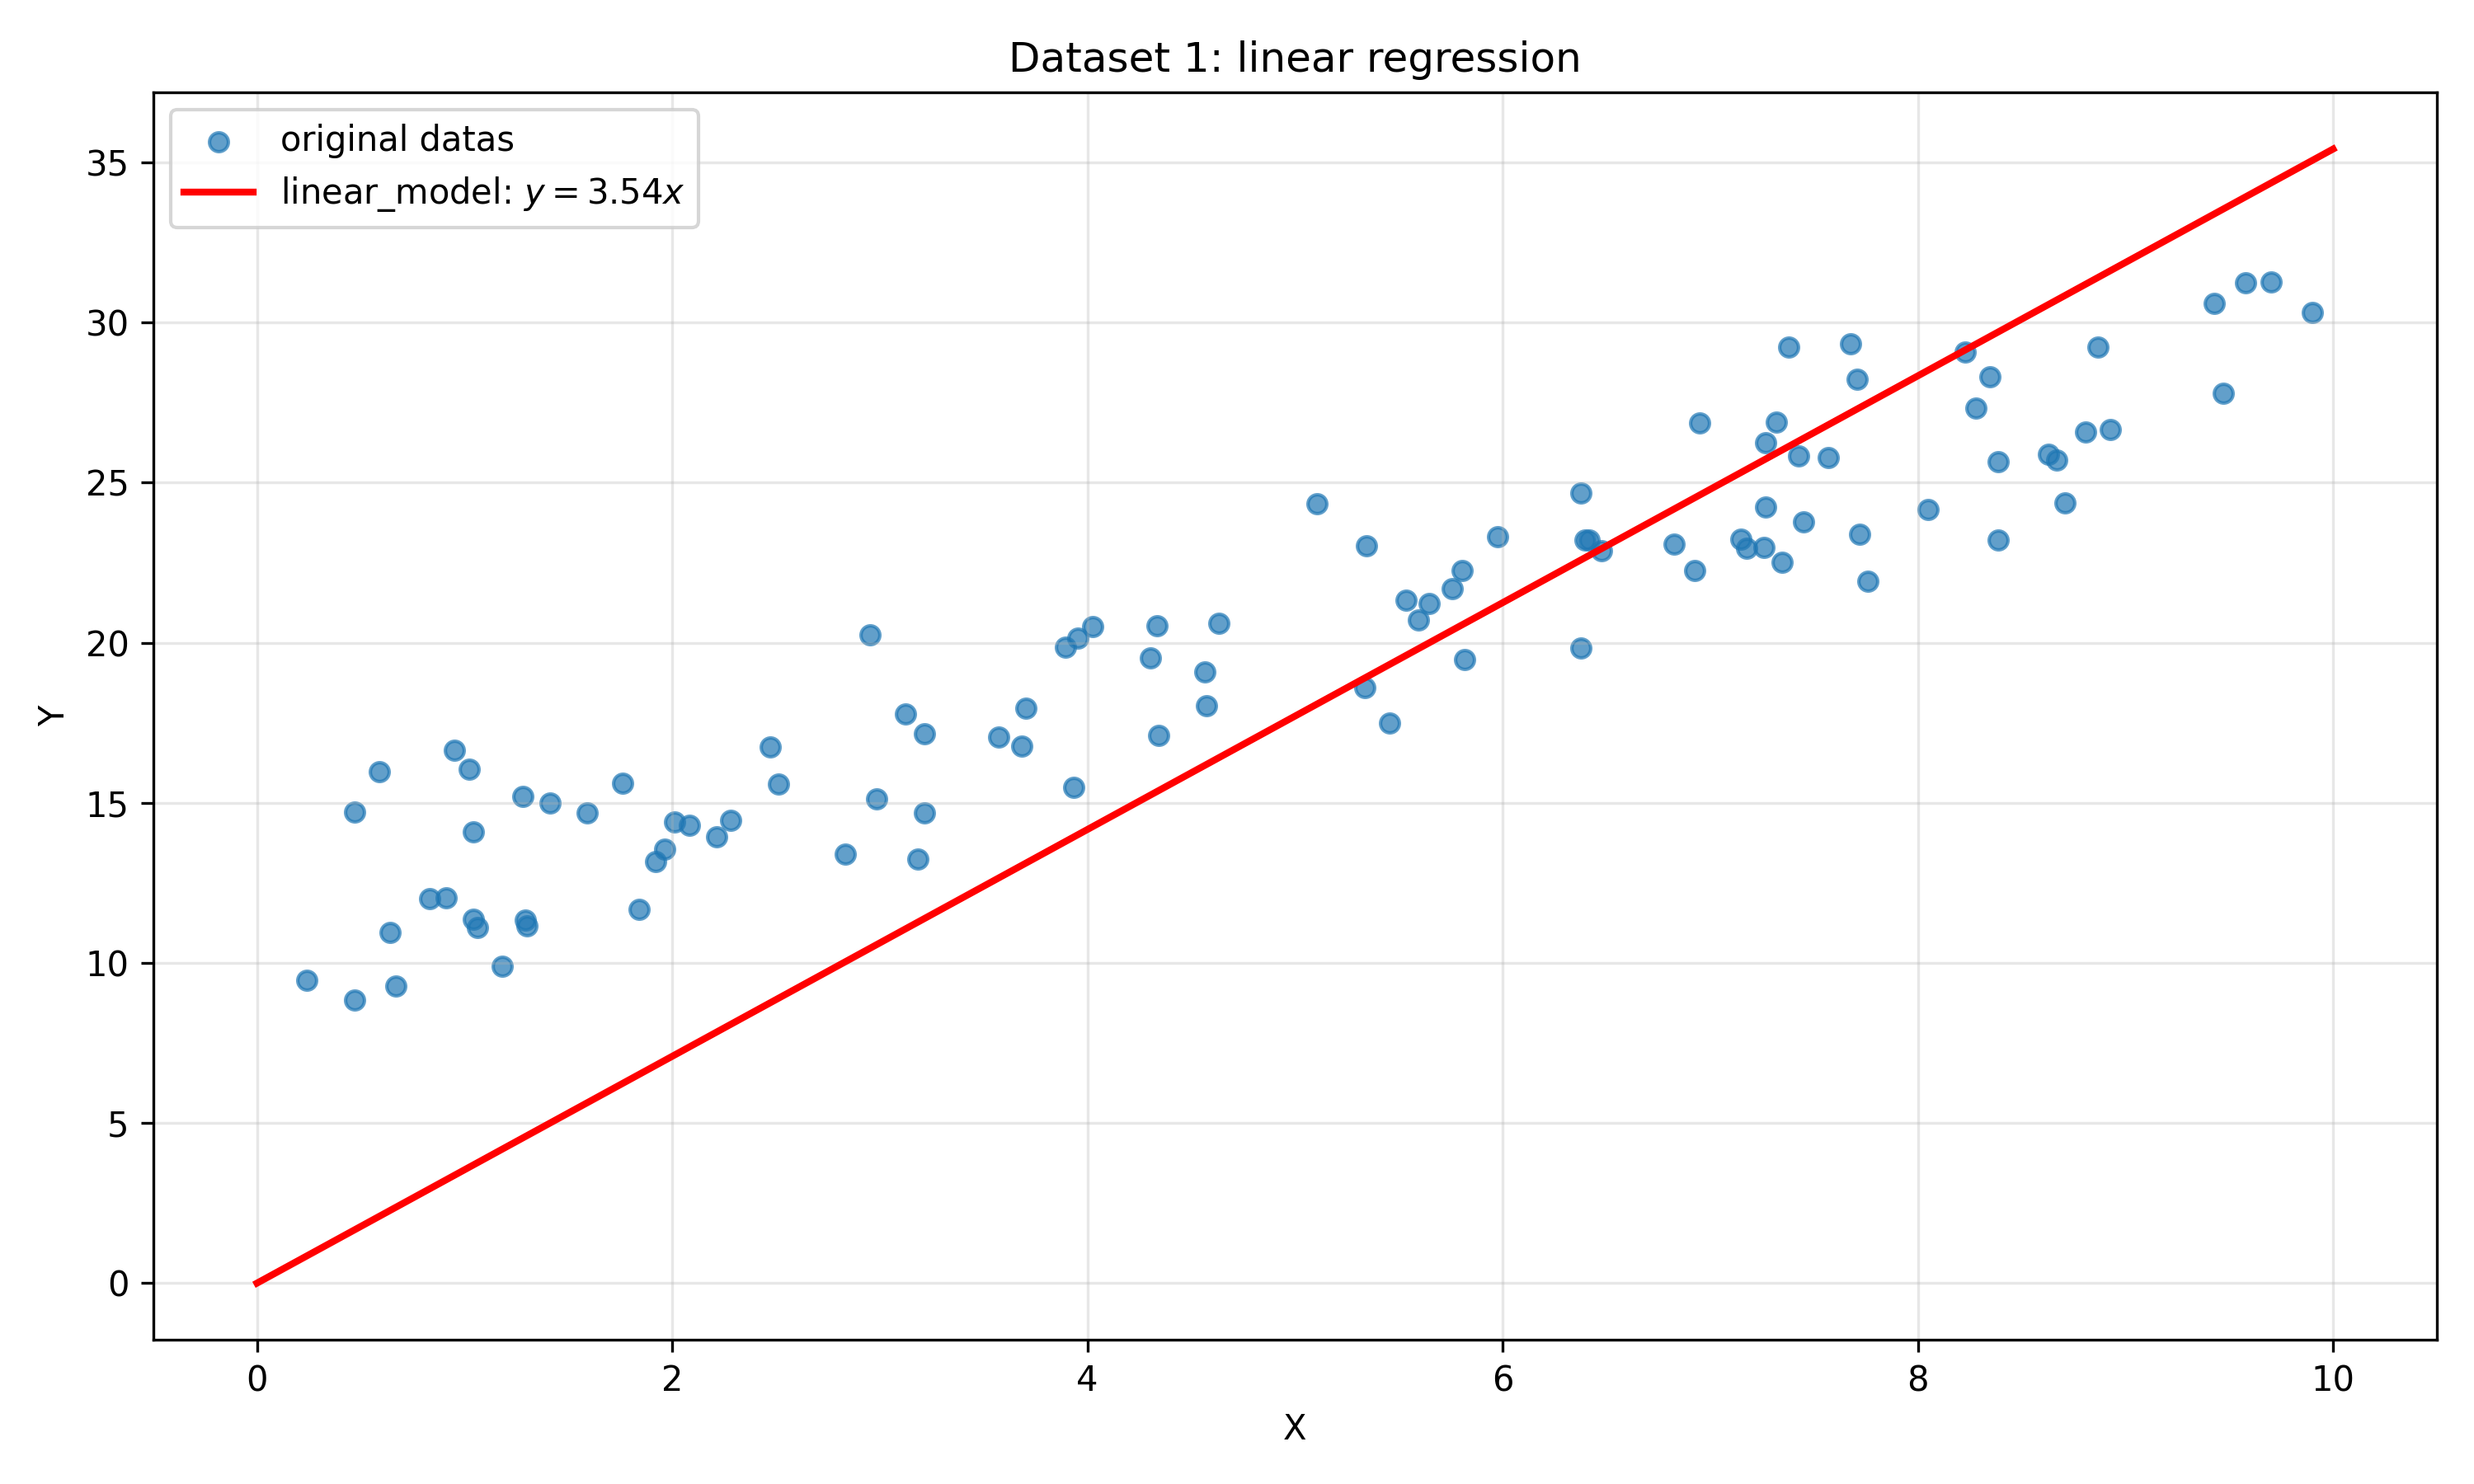
\includegraphics[width=0.8\textwidth]{problem_7c.png} 
        \caption{7c} 
        \label{fig:fig7c} 
        \end{figure}

        code: hw1\_waz.ipynb
        \[ \qedhere \]
    \end{solution}
    
    \item
    We are now going to experiment with constructing new \emph{features} for our model. 
    That is, instead of considering models that are linear in the inputs, we will now consider models that are linear in some (potentially nonlinear) transformation of the data:
    \[
        \hat{Y} = \Phi w = \begin{bmatrix}
            \phi(x_1)^\top \\
            \phi(x_2)^\top \\
            \vdots \\
            \phi(x_n)^\top
        \end{bmatrix} w,
    \]
    where $\phi(x_i), w \in \R^m$.
    Repeat part (c), providing both the mean squared error of your predictor and a plot of its predictions, for the following features on \textbf{dataset 1}:
    \[
        \phi(x_i) = \begin{bmatrix}
            x_i \\
            1
        \end{bmatrix}.
    \]
    How do the plotted function and mean squared error compare? (A single sentence will suffice.) \\
    \emph{Hint:} the general form of your solution for $w^*$ is still valid, but you will now need to use features $\Phi$ where you once used raw inputs $X$.

    \begin{solution}
        $$\mathcal{J}_\text{MSE}(w) = \frac{1}{n} \| \Phi w - Y \|_2^2.$$

        $$\nabla_w \mathcal{J}_\text{SE}(w) = (2(\Phi w-Y)^\top \Phi)^\top = 2\Phi^\top(\Phi w-Y)$$

        $\Phi^\top \Phi$ is a PSD matrix.

        $$w^* = (\Phi^\top \Phi)^{-1}\Phi^\top Y$$

        \begin{figure}[htbp]
        \centering
        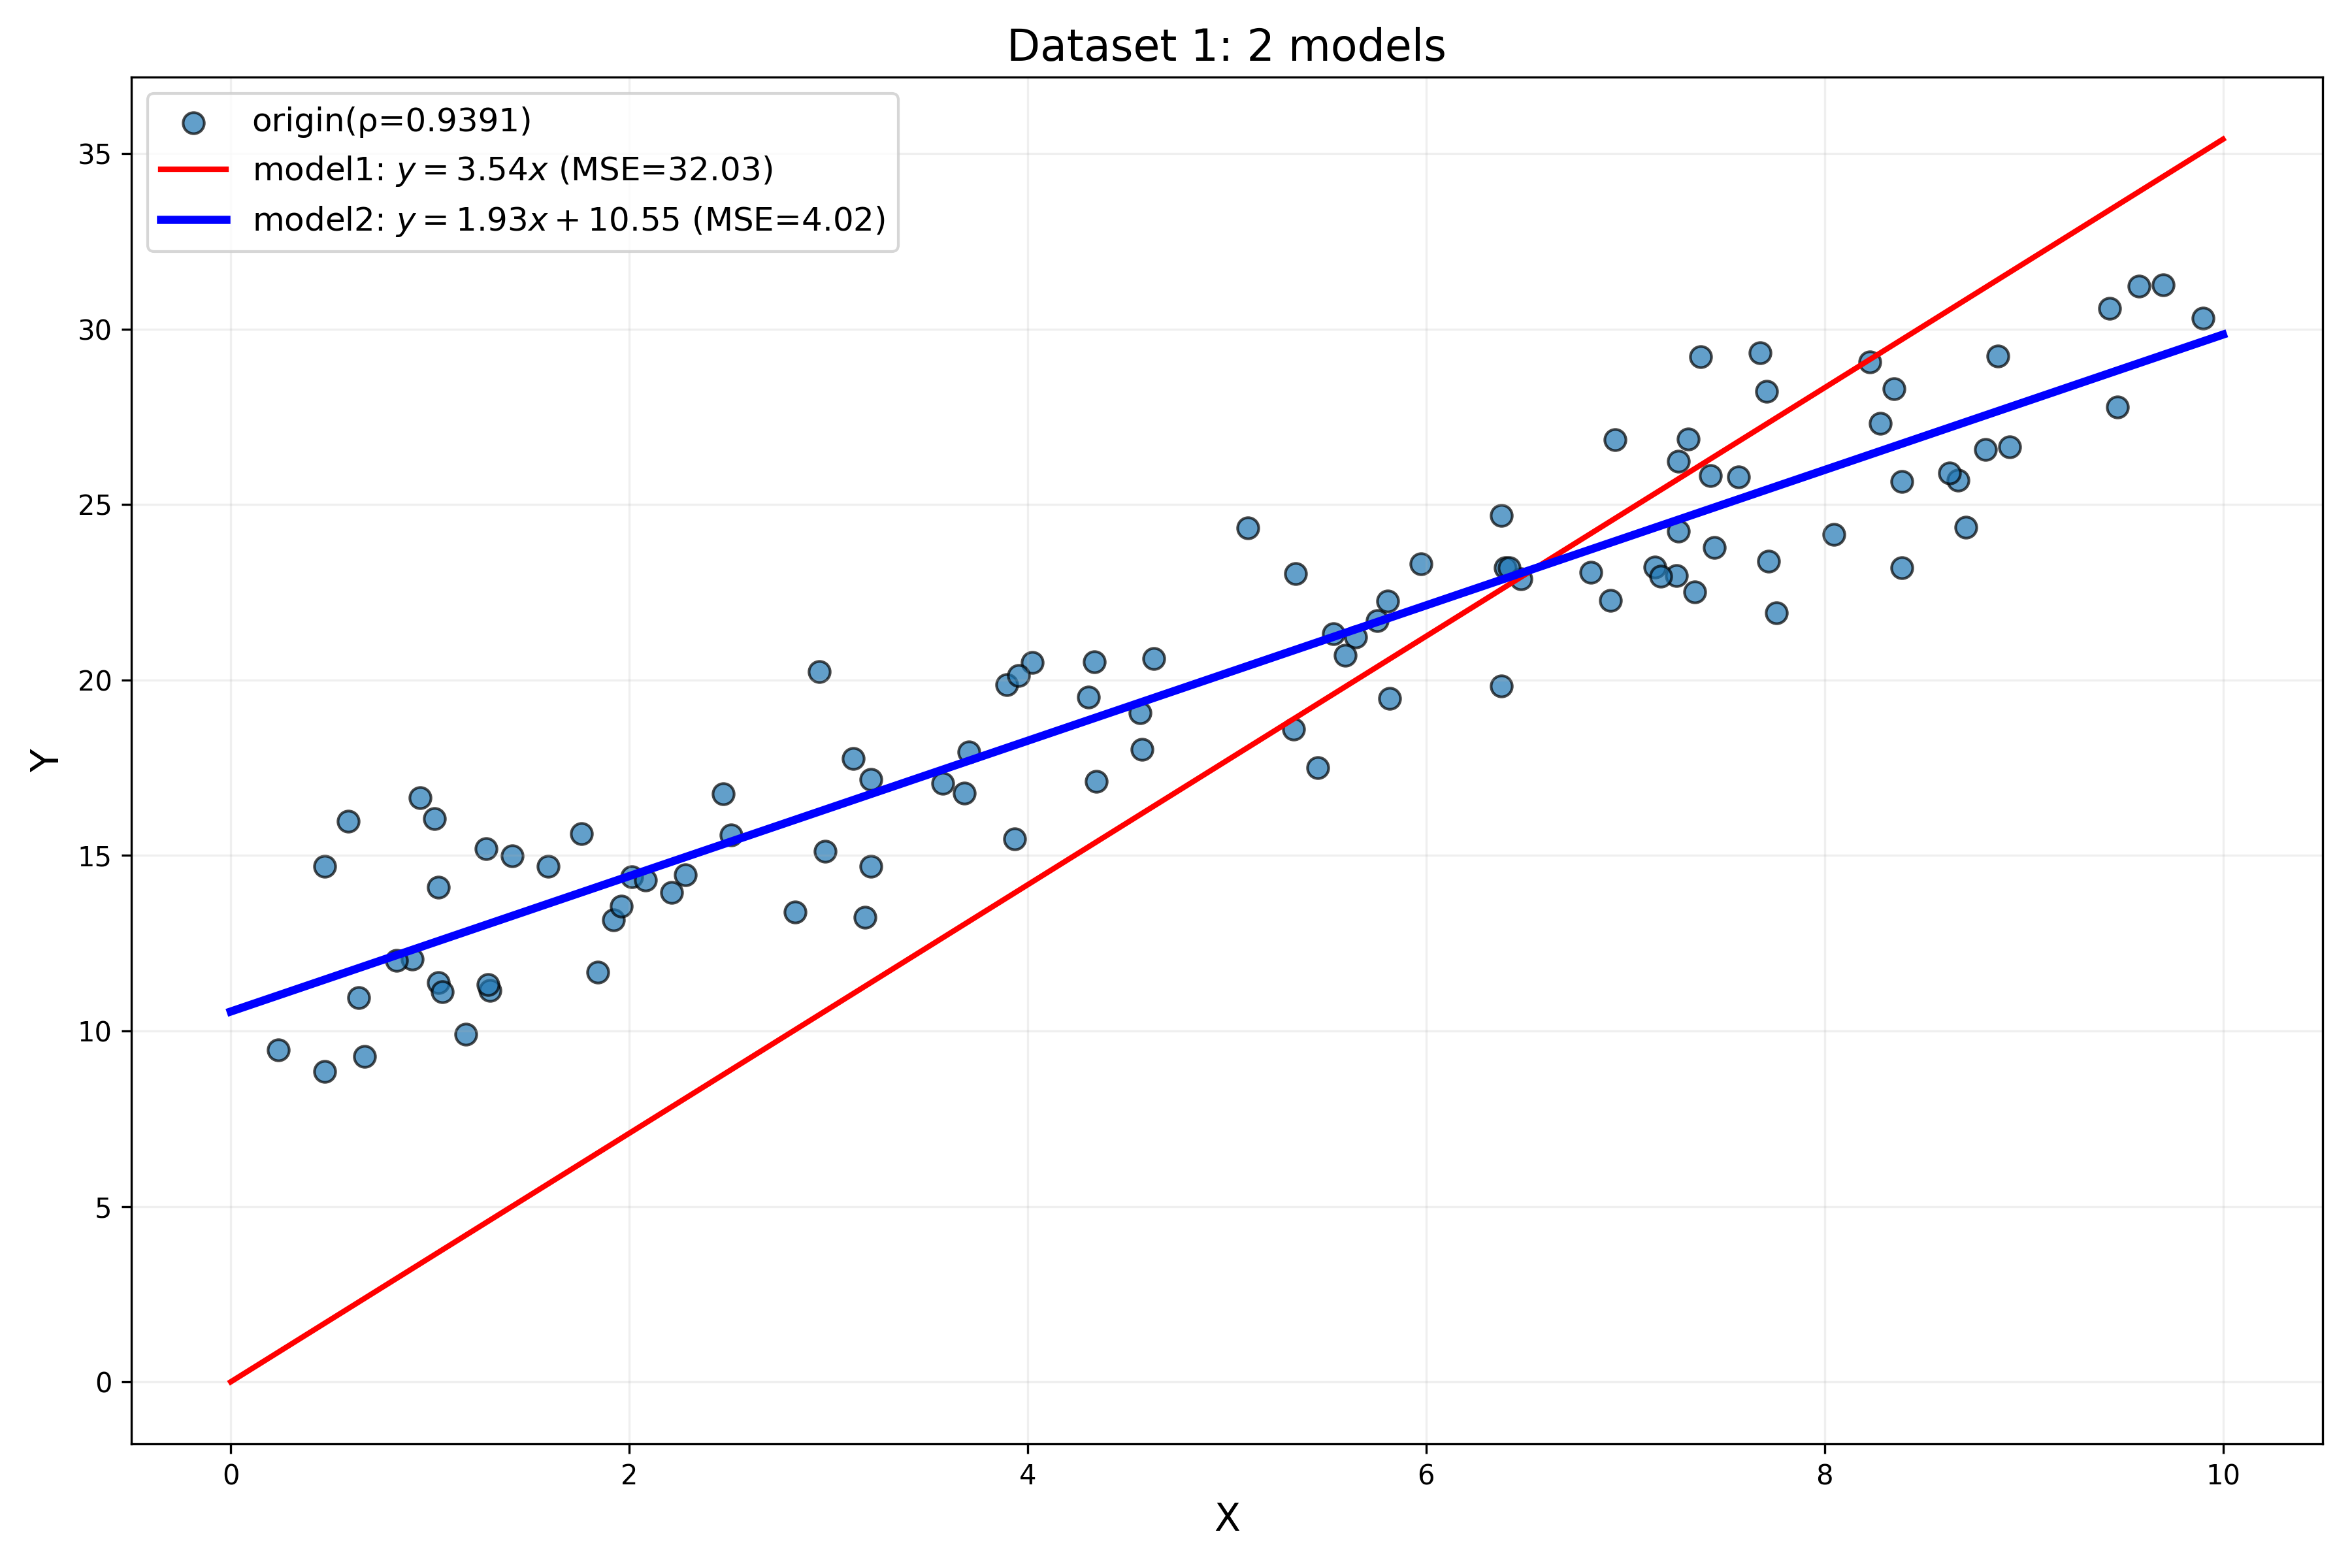
\includegraphics[width=0.8\textwidth]{problem_7d.png} 
        \caption{7d} 
        \label{fig:fig7d} 
        \end{figure}

        code: hw1\_waz.ipynb
        \[ \qedhere \]
    \end{solution}
    
    \item 
    Now consider the quadratic features:
    \[
        \phi(x_i) = \begin{bmatrix}
            x_i^2 \\
            x_i \\
            1
        \end{bmatrix}.
    \]
    Repeat part (c) with these features on \textbf{dataset 1}, once again providing short commentary on any changes.
    
    \begin{solution}

        \begin{figure}[htbp]
        \centering
        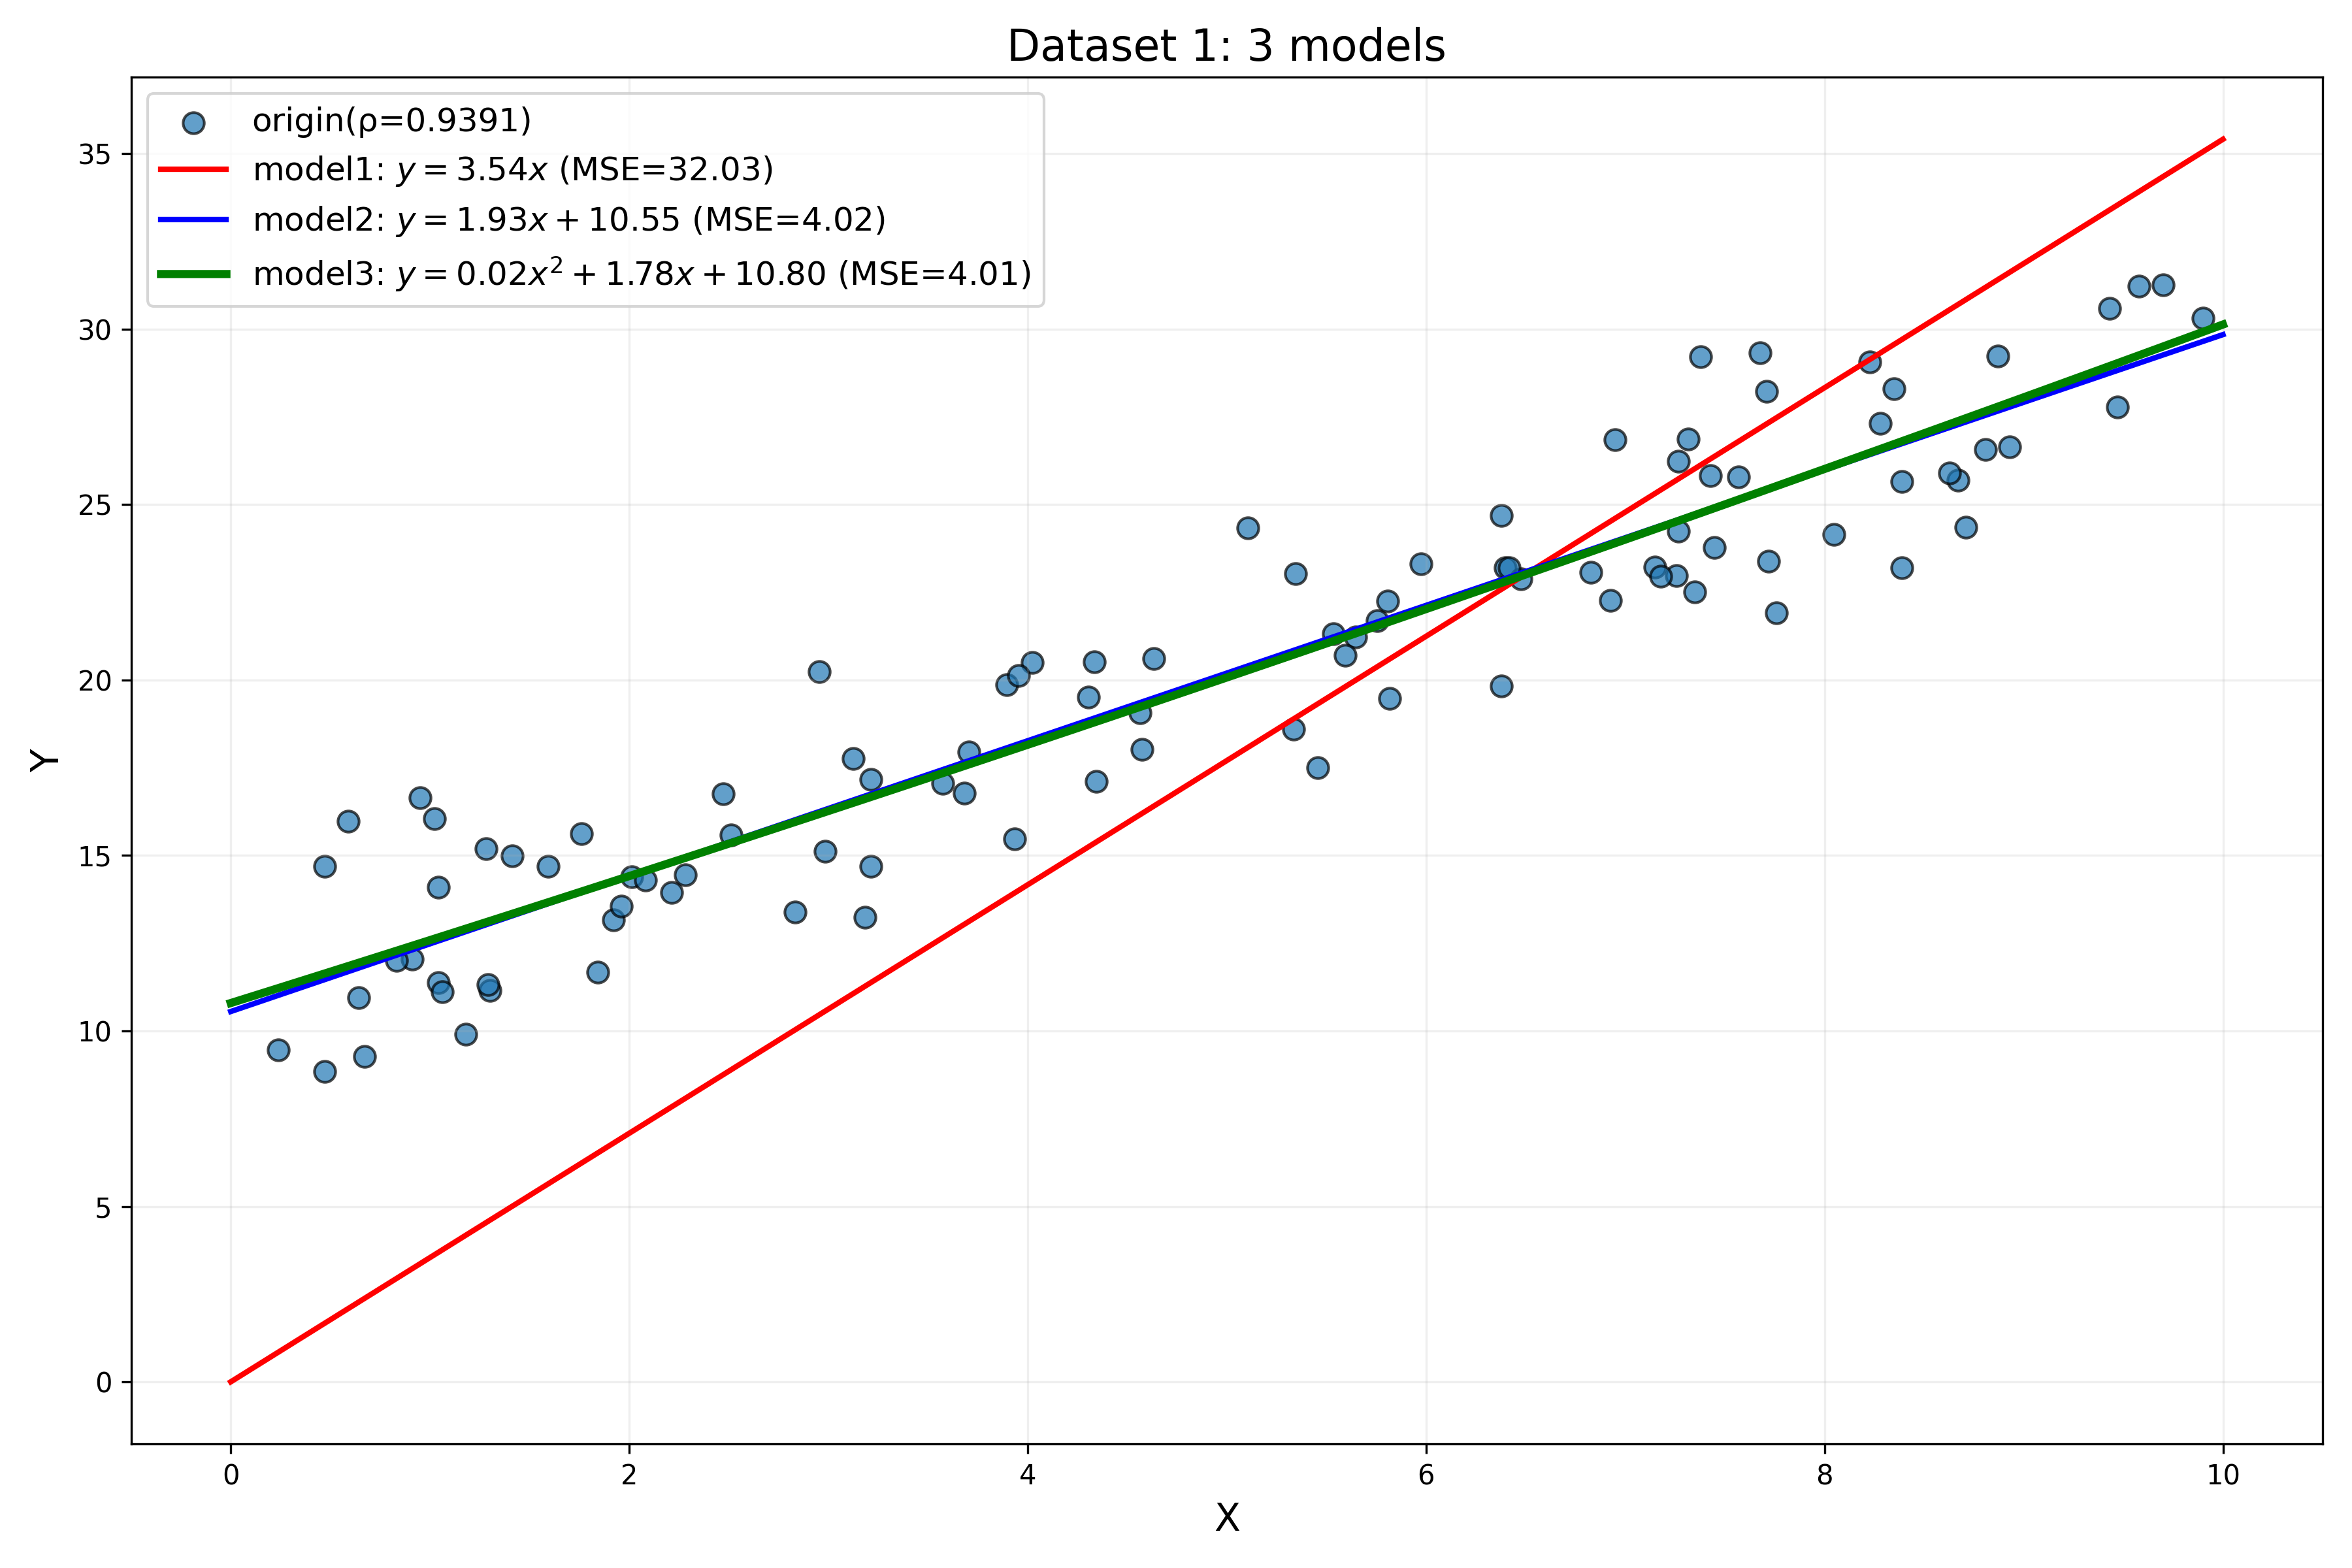
\includegraphics[width=0.8\textwidth]{problem_7e.png} 
        \caption{7e} 
        \label{fig:fig7e} 
        \end{figure}

        code: hw1\_waz.ipynb
        \[ \qedhere \]
    \end{solution}
    
    \item
    Repeat parts (c) - (e) with \textbf{dataset 2}.
    
    \begin{solution}

        \begin{figure}[H]
        \centering
        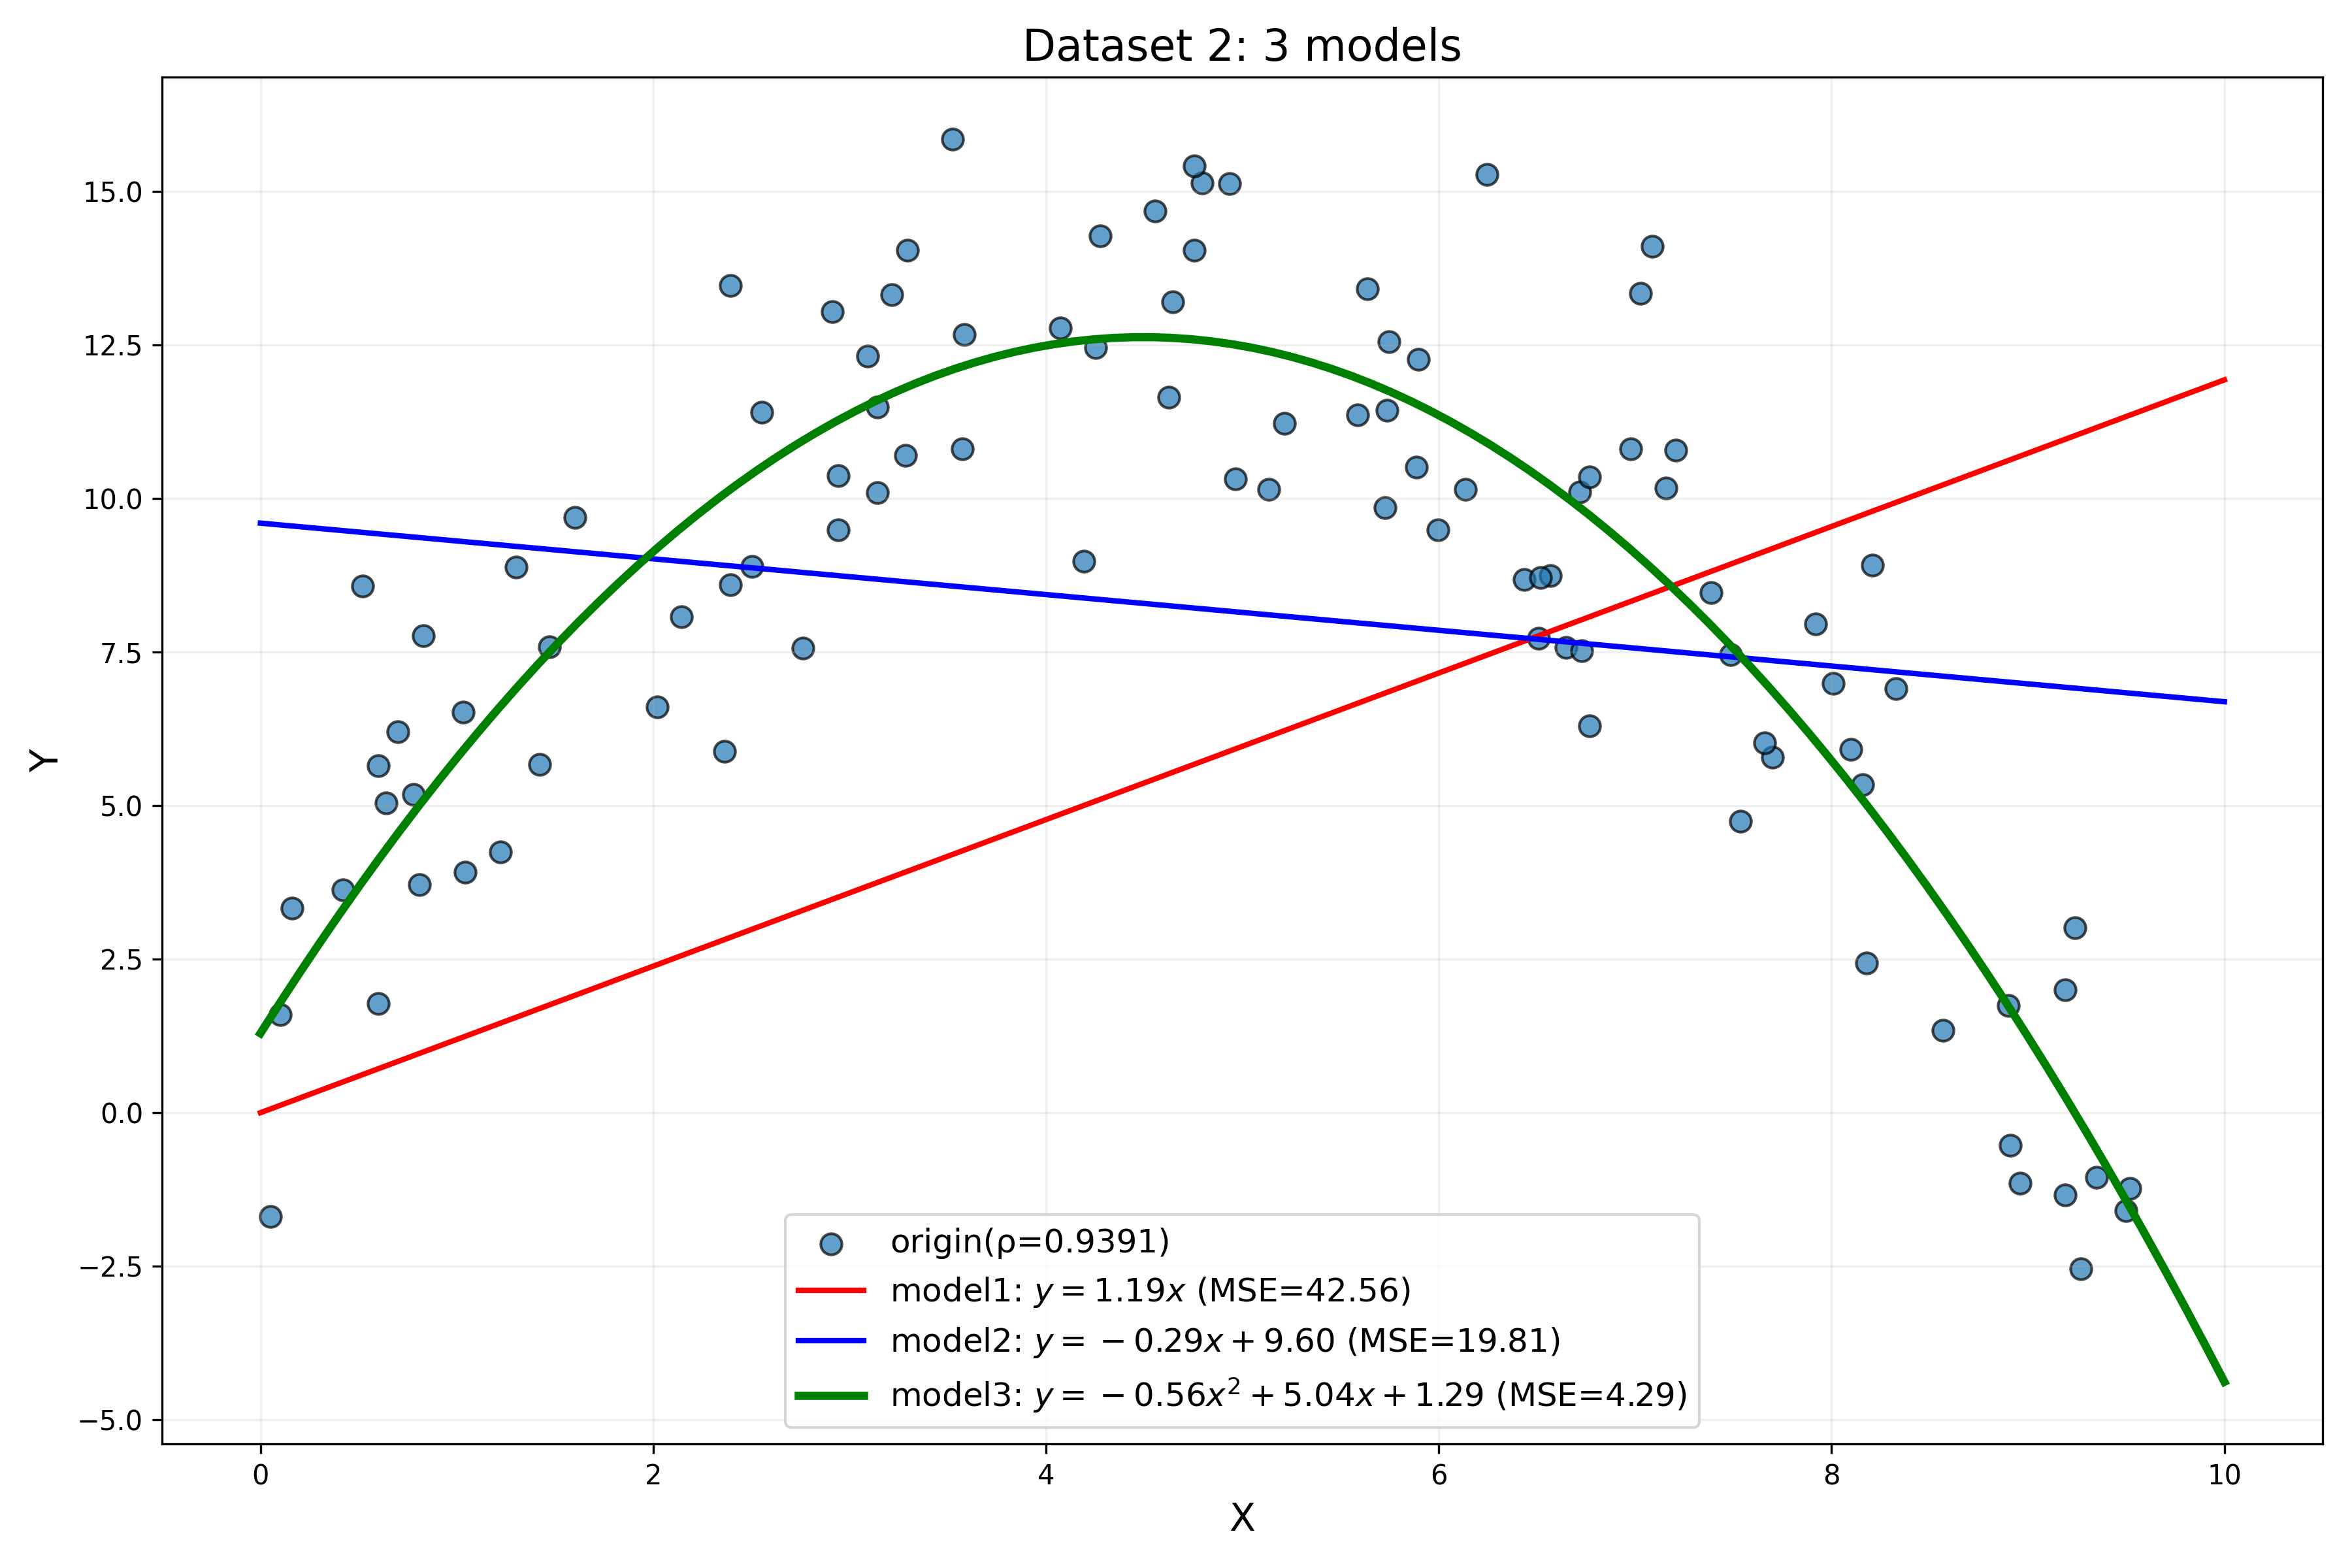
\includegraphics[width=0.8\textwidth]{problem_7f.png} 
        \caption{7f} 
        \label{fig:fig7f} 
        \end{figure}

        code: hw1\_waz.ipynb
        \[ \qedhere \]
    \end{solution}
    
    \item
    Finally, we would like to understand which features $\Phi$ provide us with the best model. 
    To that end, you will implement a method known as $k$-fold cross validation. 
    The following are instructions for this method; deliverables for part (g) are at the end.
    \begin{enumerate}[(i)]
        \item 
        Split \textbf{dataset 2} randomly into $k=4$ equal sized subsets. 
        Group the dataset into 4 distinct training / validation splits by denoting each subset as the validation set and the remaining subsets as the training set for that split.
        \item 
        On each of the 4 training / validation splits, fit linear models using the following 5 polynomial feature sets:
        \[
            \phi_1(x_i) = \begin{bmatrix}
                x_i \\
                1
            \end{bmatrix}
            ~~~~
            \phi_2(x_i) = \begin{bmatrix}
                x_i^2 \\
                x_i \\
                1
            \end{bmatrix}
            ~~~~
            \phi_3(x_i) = \begin{bmatrix}
                x_i^3 \\
                x_i^2 \\
                x_i \\
                1
            \end{bmatrix}
            ~~~~
            \phi_4(x_i) = \begin{bmatrix}
                x_i^4 \\
                x_i^3 \\
                x_i^2 \\
                x_i \\
                1
            \end{bmatrix}
            ~~~~
            \phi_5(x_i) = \begin{bmatrix}
                x_i^5 \\
                x_i^4 \\
                x_i^3 \\
                x_i^2 \\
                x_i \\
                1
            \end{bmatrix}
        \]
        This step will produce 20 distinct $w^*$ vectors: one for each dataset split and featurization $\phi_j$.        
        \item 
        For each feature set $\phi_j$, average the training and validation mean squared errors over all training splits.
    \end{enumerate}
    It is worth thinking about what this extra effort has bought us: by splitting the dataset into subsets, we were able to use all available datapoints for model fitting while still having held-out datapoints for evaluation for any particular model.

    \textbf{Deliverables for part (g):} Plot the training mean squared error and the validation mean squared error on the same plot as a function of the largest exponent in the feature set. 
    Use a log scale for the $y$-axis.
    Which model does the training mean squared error suggest is best? 
    Which model does the validation mean squared error suggest is best?

    \begin{solution}

        Degree: 1:

        Average training set MSE = 19.6999

        Average evaluating set MSE = 20.5744



        Degree: 2:

        Average training set MSE = 4.2479

        Average evaluating set MSE = 4.5649



        Degree: 3:

        Average training set MSE = 4.2024

        Average evaluating set MSE = 4.7379



        Degree: 4:

        Average training set MSE = 4.1753

        Average evaluating set MSE = 4.9702



        Degree: 5:

        Average training set MSE = 4.1589

        Average evaluating set MSE = 5.1436


        code : hw1\_waz.ipynb
        \[ \qedhere \]
    \end{solution}
    
\end{enumerate}

\newpage
\Question{Honor Code}

\begin{enumerate}
    \item 
    \textbf{List all collaborators. If you worked alone, then you must explicitly state so.}

    \begin{solution}
        Worked alone.
    \end{solution}

    \item
    \textbf{Declare and sign the following statement}: 
    
    \textit{``I certify that all solutions in this document are entirely my own and that I have not looked at anyone else's solution. I have given credit to all external sources I consulted."}
    
    \textit{Signature} : \hrulefill
    
    While discussions are encouraged, \emph{everything} in your solution must be your (and only your) creation. 
    Furthermore, all external material  (i.e., \emph{anything} outside lectures and assigned
    readings, including figures and pictures) should be cited properly.
    We wish to remind you that the consequences of academic misconduct are \emph{particularly severe}!

    \begin{solution}
        Wang Anzhe.
    \end{solution}

\end{enumerate}

\end{document}